\documentclass[10pt, mathserif]{beamer} %, mathserif
\renewcommand{\baselinestretch}{1.3}
\usepackage{bbm,tikz}
\usetheme{boxes}
\usecolortheme{rose}
\usepackage{multirow}
\setbeamertemplate{blocks}[rounded][shadow=false]
\setbeamertemplate{footline}[frame number]
\newtheorem{assumption}{Assumption}
\newtheorem{thm}{Theorem}
\newtheorem{prop}{Proposition}
\newtheorem{col}{Corollary}
\newtheorem{lem}{Lemma}
\newtheorem*{obs}{Observation}
\theoremstyle{definition}
\newtheorem{defn}{Definition}
\newtheorem{axiom}{Axiom}
\newtheorem{hyp}{Hypothesis}
\theoremstyle{plain}
\setbeamertemplate{theorems}[numbered]
\usetikzlibrary{decorations.pathreplacing}
\newenvironment{sequation}{\small\begin{equation}}{\end{equation}}
\newenvironment{sequation*}{\small\begin{equation*}}{\end{equation*}}
\newenvironment{tequation}{\tiny\begin{equation}}{\end{equation}}
\newenvironment{tequation*}{\tiny\begin{equation*}}{\end{equation*}}
\usepackage{pstricks,egameps}


\def\trueB{\mB^{\text{true}}}
\def\newX{\mX_{\textup{new}}}
\def\newy{y_{\textup{new}}}
\def\sign{\textup{sgn}}

\def\srank{\textup{srank}}
\def\rank{\textup{rank}}
\def\caliP{\mathscr{P}_{\textup{sgn}}}
\def\risk{\textup{Risk}}
 \definecolor{darkgreen}{rgb}{0.0, 0.4, 0.1}

\newcommand*{\KeepStyleUnderBrace}[1]{%f
\mathop{%
\mathchoice
{\underbrace{\displaystyle#1}}%
{\underbrace{\textstyle#1}}%
{\underbrace{\scriptstyle#1}}%
{\underbrace{\scriptscriptstyle#1}}%
}\limits
}
\usepackage{pifont}
\usepackage{pgfpages}
\usepackage[ruled]{algorithm2e}

\setbeameroption{hide notes}
\setbeamertemplate{note page}{%
  \insertnote%
}
\usepackage{lmodern}
\setlength{\leftmargini}{0pt}
\setlength{\leftmarginii}{14pt}

\usepackage{dsfont}
\usepackage{wrapfig}
\usepackage{mathrsfs}

\def\caliP{\mathscr{P}_{\textup{sgn}}}


\usepackage{mathtools}
\mathtoolsset{showonlyrefs}
\usepackage{appendixnumberbeamer}
\usepackage{appendix}

\usepackage{natbib}
\usepackage{graphicx}
\usepackage{setspace}

\usepackage{empheq}
\title[Higher-order tensors]{\\
\vspace{1.5cm}
Beyond matrices: nonparametric tensor completion via sign series}
\author{Miaoyan Wang\\}
\date{}
\institute{
{\scriptsize
Department of Statistics, UW-Madison\\
\vspace{.4cm}
}
{\scriptsize
Joint work with Chanwoo Lee (3rd-year PhD student)\\
\vspace{.2cm}
\\
}
\hspace{8cm}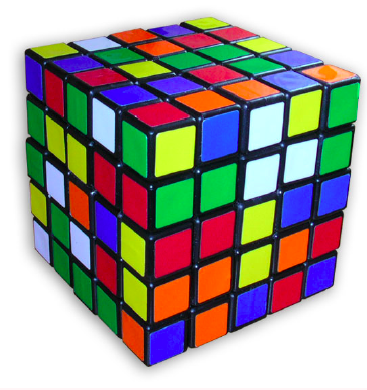
\includegraphics[width=2cm]{Figures/image.png}
\\
}

    
\AtBeginSection[]

\usepackage{bm}
\input macros.tex

\begin{document}
\renewcommand{\raggedright}{\leftskip=0pt \rightskip=0pt plus 0cm}

\begin{frame}[plain]{}{}
\titlepage
\end{frame}


%\begin{frame}[plain]{Research in my group}

%{\bf Statistical machine learning:}
%\begin{itemize}
%\item Structured tensor decomposition, latent factor models
%\end{itemize}
%\bigskip
%\bigskip

%{\bf Genetics and genomics:}
%\begin{itemize}
%\item gene expression analyses, genetic association studies
%\end{itemize}
%\bigskip
%\bigskip

%{\bf Foundations of data science:}
%\begin{itemize}
%\item Statistical-computational tradeoff for big data analytics 
%\end{itemize}
%\end{frame}

\begin{frame}{A successful story: PCA of Europeans}

\centerline{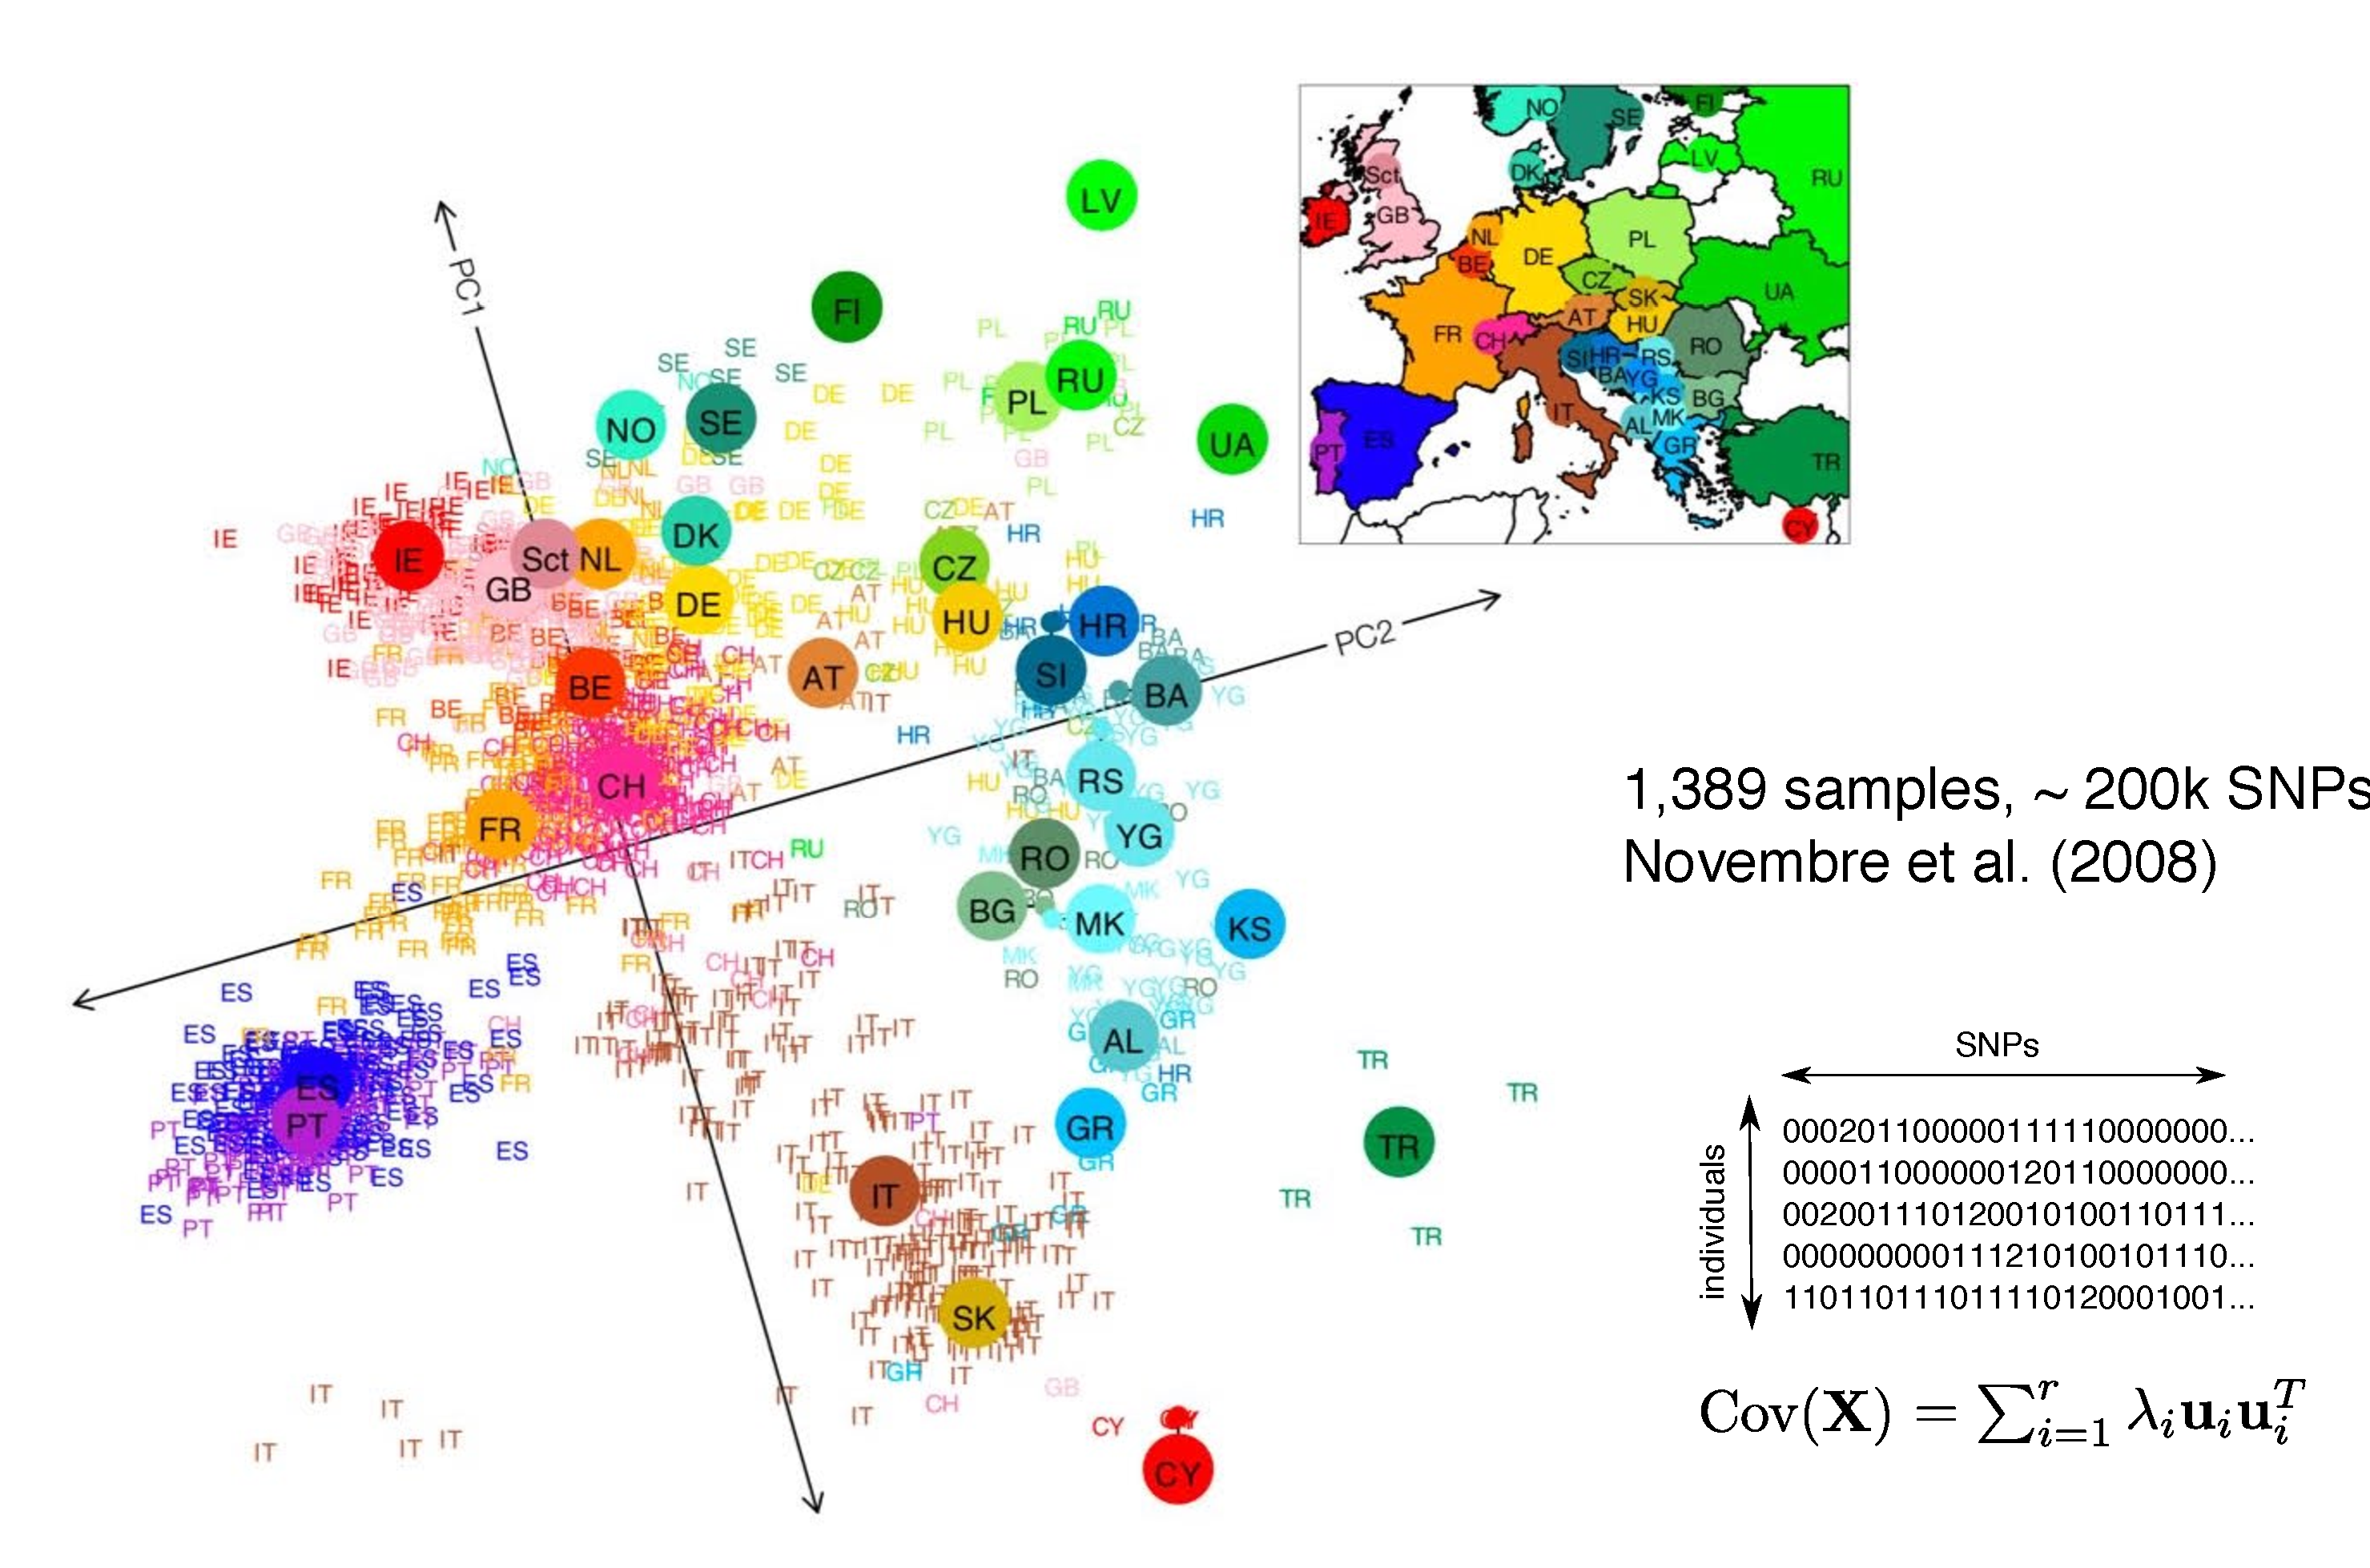
\includegraphics[width=1\textwidth]{Figures/SNP.pdf}}
\end{frame}


\begin{frame}{Matrix methods are powerful, however...}

\centerline{ 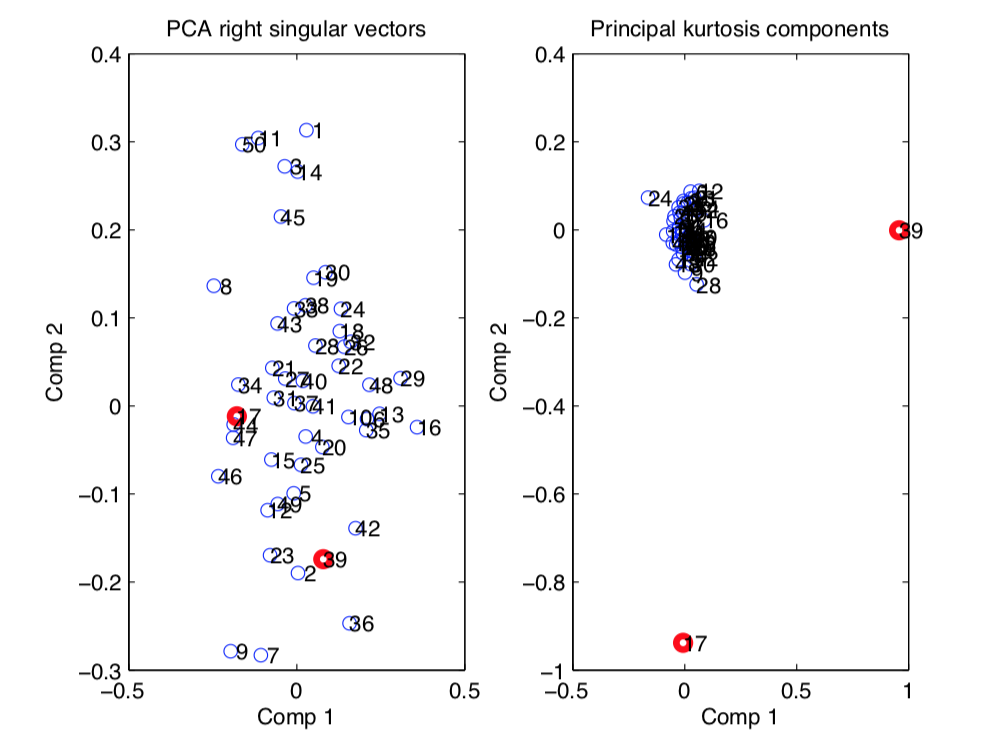
\includegraphics[width=.7\textwidth]{Figures/PCA.png}}

All Gaussian except points 17 and 39. 

left: matrix PCA;  right: principal components of kurtosis.

{\scriptsize Figure credit: Jason Morton and Lek-Heng Lim (2009/2015).}
\end{frame}


\begin{frame}{What is a tensor?}

\begin{itemize}

\item Tensors are generalizations of vectors and matrices:

\onslide 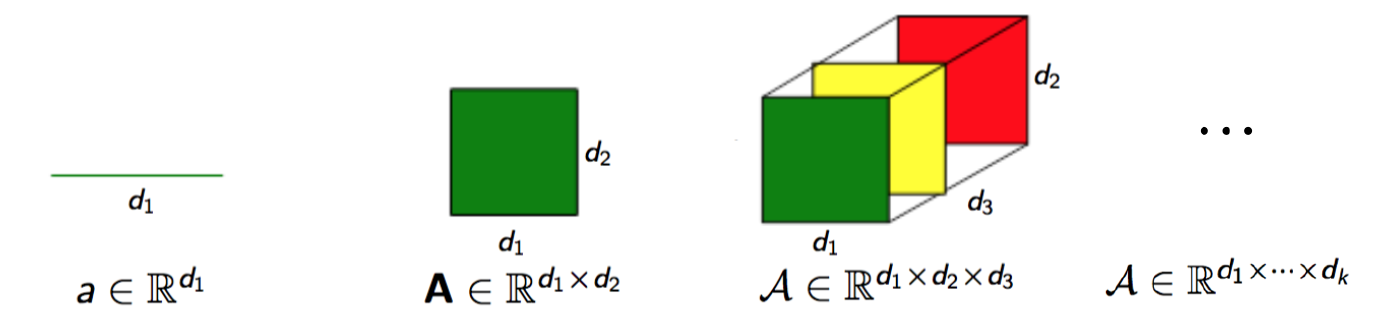
\includegraphics[width=.9\textwidth]{Figures/defn.png}
\item An order-$k$ tensor $\tensor{A} = \entry{a_{i_1\dots\, i_k}}  \in \mathbb{R}^{d_1 \times \dots \times d_k}$ is a hypermatrix with dimensions $(d_1,\ldots,d_k)$ and entries $a_{i_1\dots i_k}\in\mathbb{R}$.
\item This talk will focus on tensor of order $3$ or greater, also known as \red{higher-order tensors}.
\end{itemize}
\end{frame}

\begin{frame}{Tensors in genomics}

\begin{itemize}
\item Many datasets come naturally in a multiway form.
\item Multi-tissue, multi-individual gene expression measures could be organized as an order-3 tensor $\tA=\entry{a_{git}}\in \mathbb{R}^{n_G\times n_I\times n_T}$.
\end{itemize}
\bigskip
\centerline{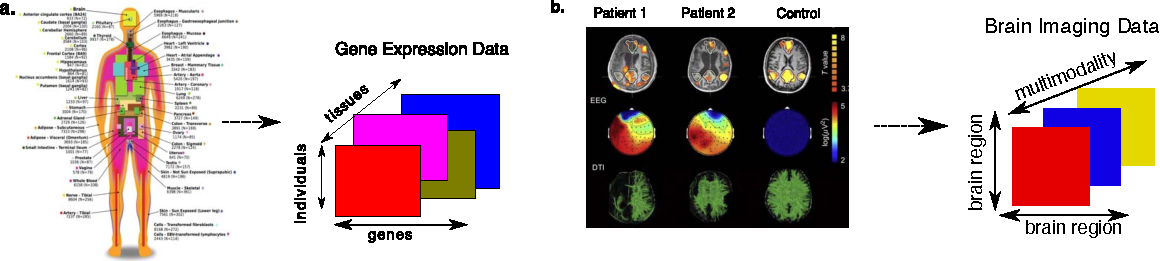
\includegraphics[width=\textwidth]{Figures/example.pdf}}
\bigskip
\end{frame}


\begin{frame}{Tensors in statistical modeling}
``Tensors are the new matrices'' that tie together a wide range of areas:
\bigskip
\begin{itemize}
\item Longitudinal social network data $\{\mY_t: t=1,...,n\}$
\item Spatio-temporal transcriptome data
\item Joint probability table of a set of variables $\mathbb{P}(X_1,X_2,X_3)$
\item Higher-order moments in topic models
\item Markov models for the phylogenetic tree $K_{1,3}$
\end{itemize}
\bigskip
\hfill {\scriptsize M. Yuan et al 2017, P. Hoff 2015, Montanari \& Richard 2014}\\
\hfill{\scriptsize  Anandkumar et al 2014, Mossel et al 2004, P. McCullagh 1987}
\end{frame}


\begin{frame}[noframenumbering]{Talk outline} 
 \begin{alertblock}{Prohibitive Computational Complexity}
Most higher-order tensor problems are NP-hard [Hillar \& Lim, 2013].
\end{alertblock}


\begin{columns}[T] \begin{column}{.4\textwidth}
\centering
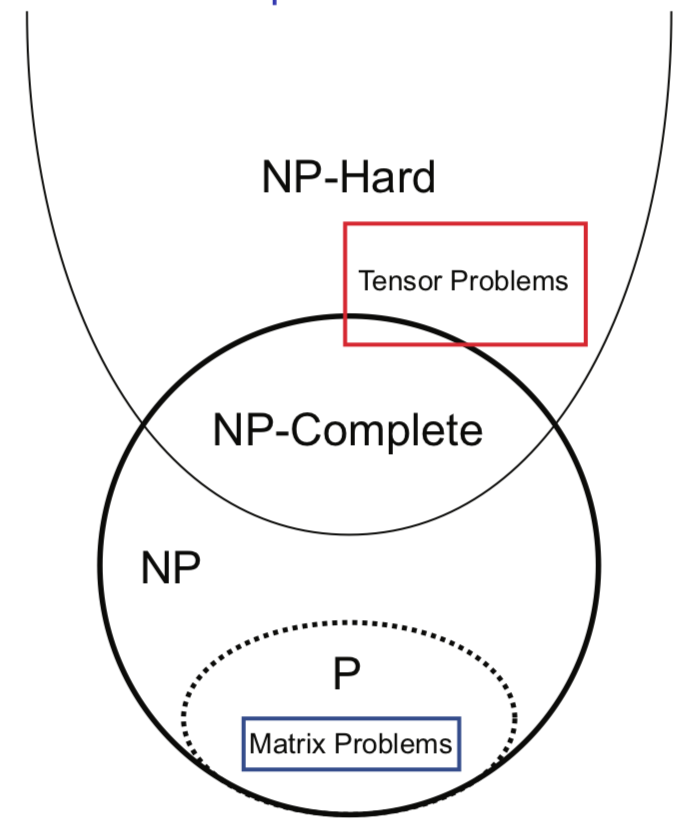
\includegraphics[width=3cm]{Figures/NP.png}
\end{column}%
\hfill%
\begin{column}{.6\textwidth}
Fortunately, the tensors sought in statistical and machine learning applications are often \color{red}specially structured:
\begin{itemize}
\item Low-rankness
\item Sparsity
\item Non-negativity
\item ...
\end{itemize}
\end{column}%
\end{columns}

\begin{block}{This talk is based on}
{\footnotesize {\color{blue}Beyond the Signs: Nonparametric Tensor Completion via Sign Series.} Lee and W. 2021
\url{https://arxiv.org/pdf/2102.00384.pdf}}
\end{block}
\end{frame}


\begin{frame}[label=matrix]{Review: Matrix SVD for biclustering}
\vspace{.2cm}

\centerline{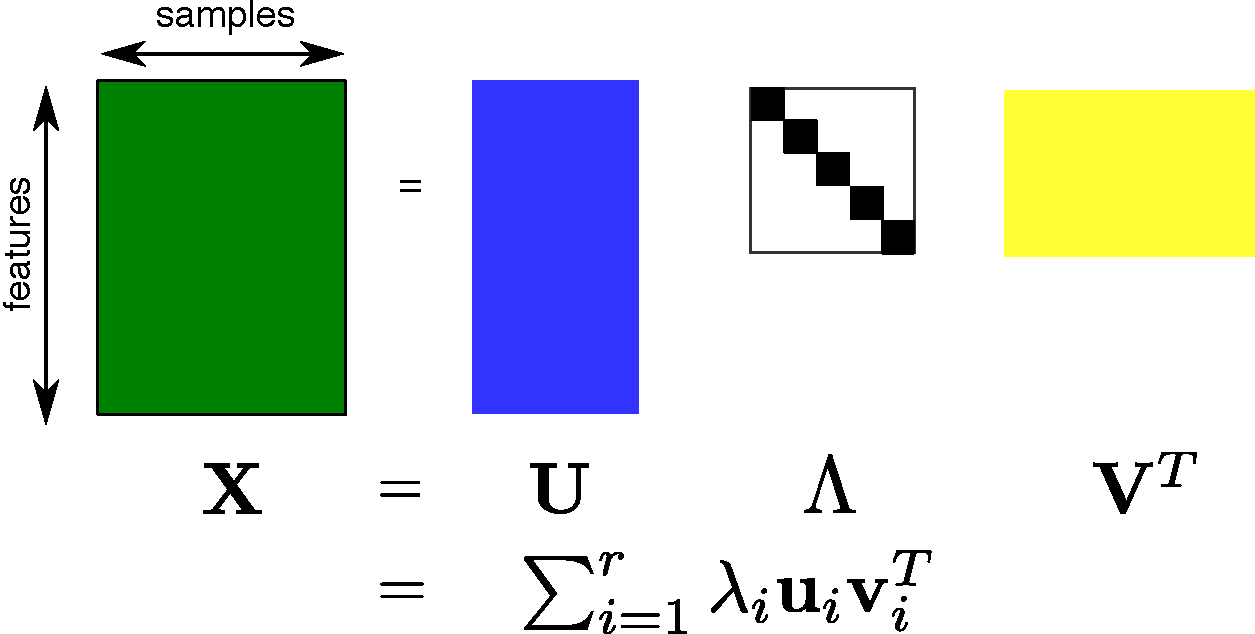
\includegraphics[width=.9\textwidth]{Figures/svd.pdf}}

\begin{itemize}
\item Columns of ${\bf U}$ describe patterns across samples
\item Columns of ${\bf V}^T$ describe patterns across genes
\end{itemize}

\setstretch{0.6}{
{\hfill \tiny Y Kluger et al, Genome Research (2003). 13(4): 703-71}\\
{\hfill \tiny Data Science Specialization (COURSERA) by Brian Caffo and Jeff Leek}\\
}

 
\end{frame}


\begin{frame}{Various notions of low-rankness}
\begin{itemize}
\item Canonical polyadic (CP) low-rankness: $\tA=\sum_{r=1}^R\lambda_r\ms_r\otimes \mg_r\otimes \mt_r$.

\vspace{.3cm}
\centerline{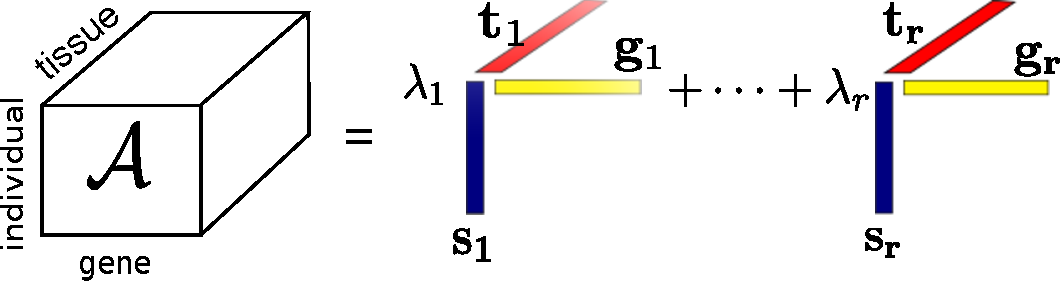
\includegraphics[width=7cm]{Figures/CP_decomp2.pdf}}

\item Tucker low-rankness: $\tA=\tC\times_1\mS\times_2 \mG\times_3\mT$.

\vspace{.5cm}
\centerline{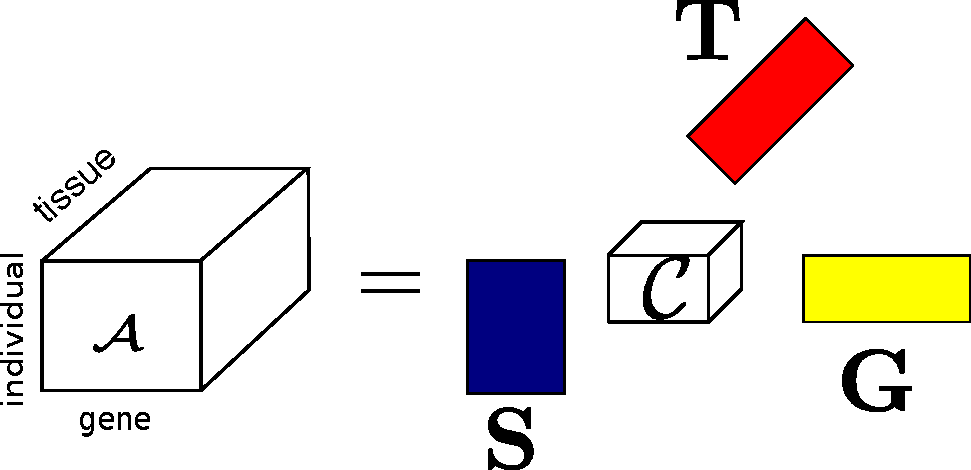
\includegraphics[width=6cm]{Figures/HOSVD.pdf}}
\item Others: tensor train {\scriptsize[Oseledet '11]}, tensor block model {\scriptsize[W. \& Zeng '19; Han, Luo, W. et al '20]}, etc.
\end{itemize}
\end{frame}


\begin{frame}{Setup: signal plus noise model}
     \begin{center}
    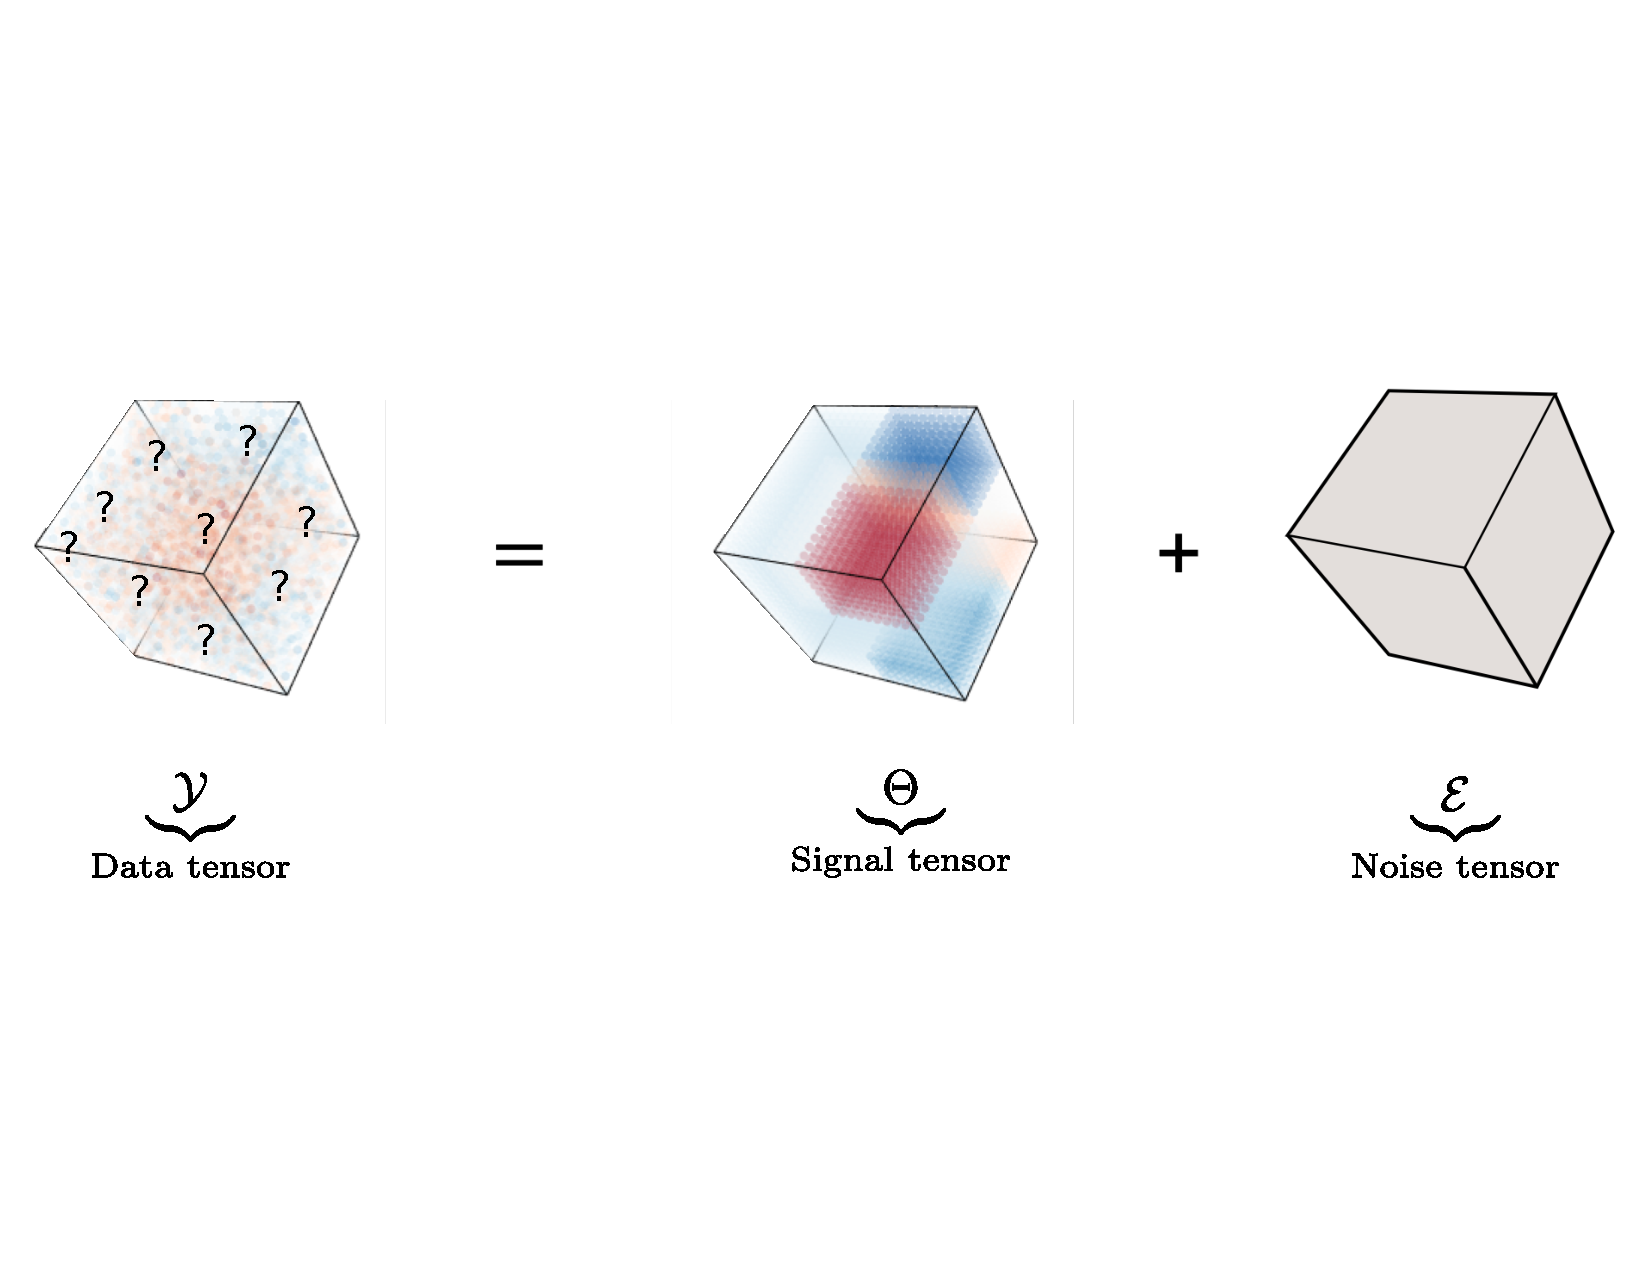
\includegraphics[width =\textwidth]{Figures/signalnoise.pdf}
    \end{center}
    We focus on two problems:
    \begin{itemize}
        \item Nonparametric tensor estimation: How to estimate the signal tensor $\Theta$ under {\color{red}a wide range of structures}?
        \item Tensor completion: How many {\color{red}observed tensor entries} do we need in order for consistent recovery?
    \end{itemize}
\end{frame}

\begin{frame}{Inadequacies of low-rank models}
 \begin{itemize}
 \item Classical low-rank models (Jain \& Oh '14; Motanari \& Sun '18):
 \\[.5cm]

   \begin{center}
    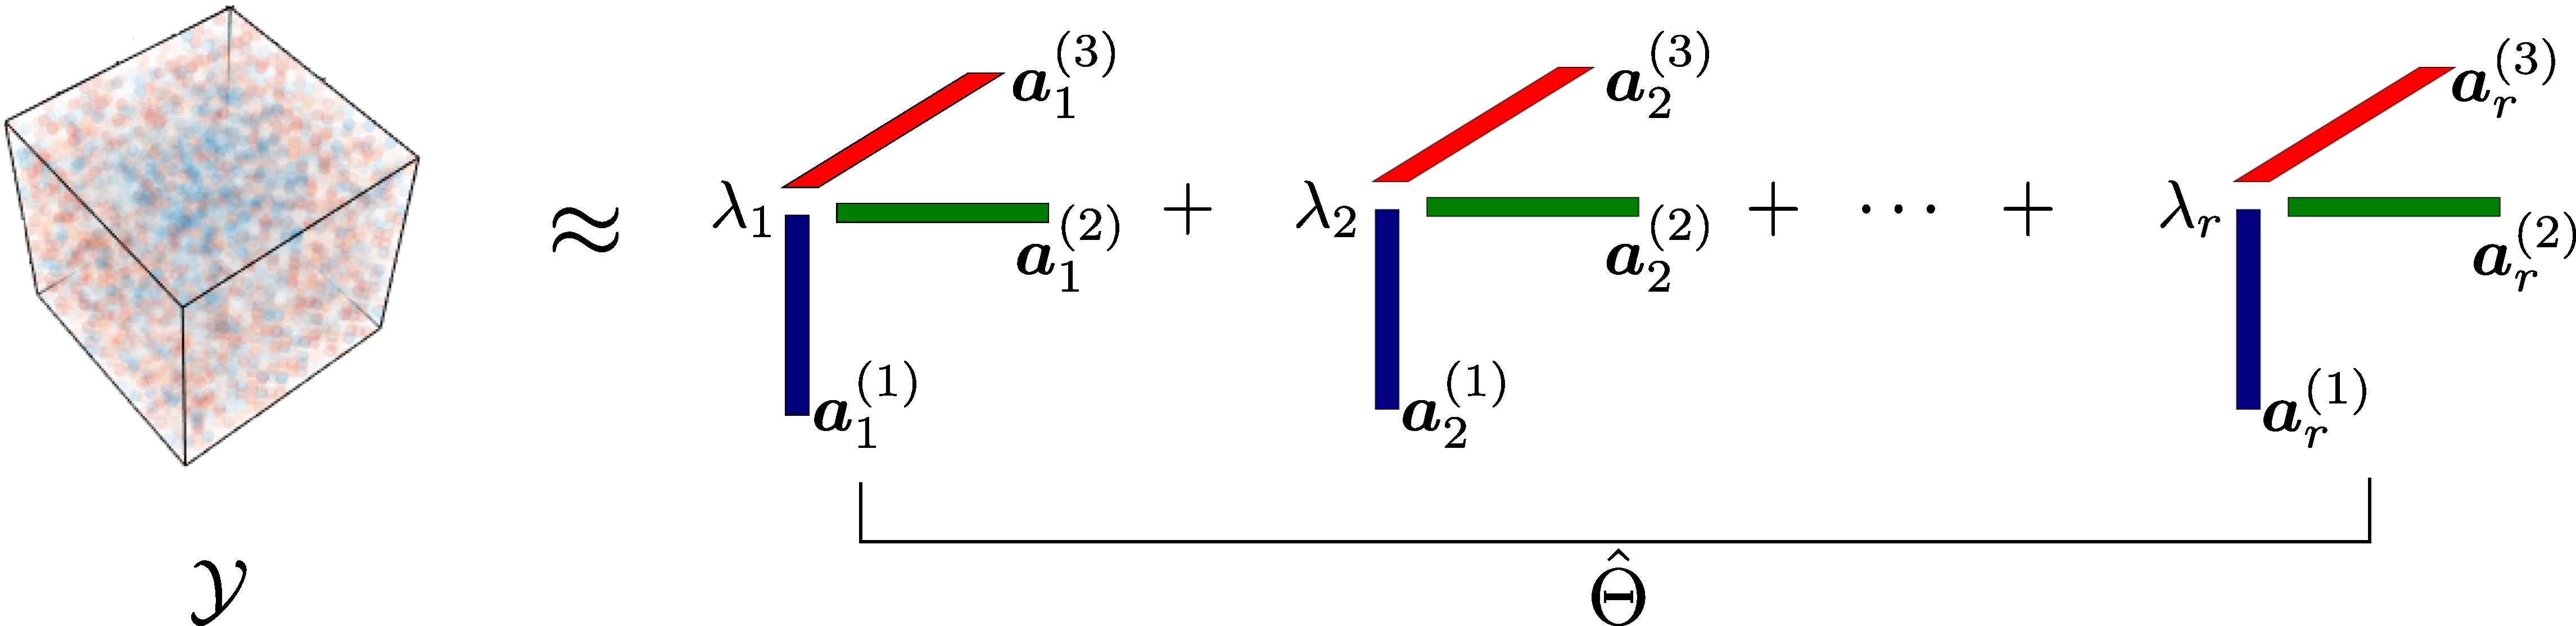
\includegraphics[width =\textwidth]{Figures/classic.pdf}
    \end{center}

     \item Two limitations of classical low-rank models:
     \begin{enumerate}
         \item Sensitivity to order-preserving transformation.
         \item Inadequacy for special structures.
     \end{enumerate}
 \end{itemize}
\end{frame}

\begin{frame}{Inadequacies of  low-rank models}
 \begin{itemize}         
  \item Tensor rank is sensitive to order-preserving transformation.
\begin{columns}
\begin{column}{0.5\textwidth}
   \begin{center}
     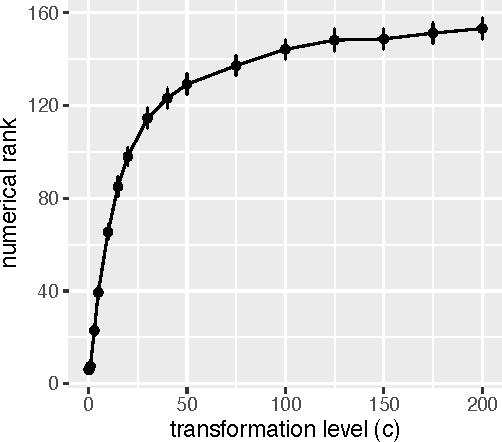
\includegraphics[width=0.7\textwidth]{Figures/example1.pdf}
     \end{center}
\end{column}
\begin{column}{0.6\textwidth} 
\begin{align}
\Theta &= {1\over 1+\exp(-c\left(\mathcal{Z}\right))},\quad\text{where }\\ 
\tZ &= \bm a^{\otimes3}+ \bm b^{\otimes3}+ \bm c^{\otimes3}
\end{align}
$\Rightarrow$ $\Theta$ is high-rank but $\tZ$ is low-rank. 
\end{column}
\end{columns}
      
   \pause   
   
 \item Low-rank model fails to address several important structures.
 \begin{columns}
\begin{column}{0.55\textwidth}
   \begin{center}
     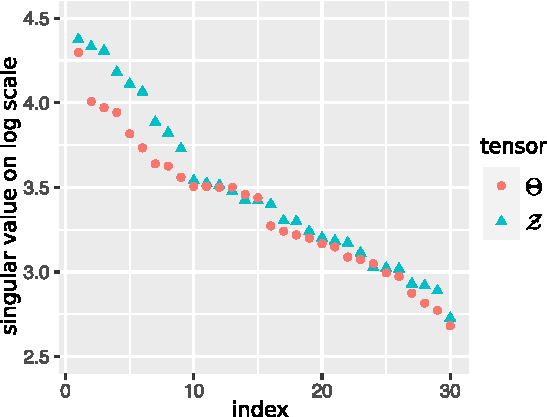
\includegraphics[width=0.7\textwidth]{Figures/example2.pdf}
     \end{center}
\end{column}
\begin{column}{0.6\textwidth}  
\begin{align}\Theta &= \log(1+\mathcal{Z}),\quad\text{ where }\\
\tZ&=\entry{\mathcal{Z}(i,j,k)}  = \frac{1}{d}\max(i,j,k). \text{ }\hspace{1cm} 
\end{align}
$\Rightarrow$ Both $\Theta$ and $\tZ$ are full rank. 
\end{column}
\end{columns}
    
{\tiny \hfill The matrix analogy of $\Theta$ was studied in the context of graphon analysis by Chan \& Airoldi '14.}
 \end{itemize}
\end{frame}


\begin{frame}{Related work and our contributions}


\begin{itemize}
\item {\bf Low-rank tensor estimation} (Anandkumar et al.\ '14; Montanari \& Sun '18; Cai et al.\ '19) focuses on the regime of fixed rank $r$ growing dimension $d$. $\Rightarrow$ {\color{red}low-rank assumption is often violated} in practice. 
\item {\bf High-rank matrix estimation} was studied under nonlinear models (Ganti et al.\ '15) and subspace clustering (Ongie et al.\ '17; Fan \& Udell '19). $\Rightarrow$ tensors are more challenging because {\color{red}tensor rank may exceed dimension}. 
\end{itemize}

\pause
\begin{block}{Our contributions}
\begin{itemize}
\item We develop a new model called {\color{red} sign representable tensors} to fill the gap between parametric (low-rank) and nonparametric (high-rank) tensors. 
\item Our tensor estimate is {\color{red}provably reductable} to a series of classifications. $\Rightarrow$ computationally efficient via a divide-and-conquer algorithm. 
\end{itemize}
\end{block}
\end{frame}

\begin{frame}{Why sign matters?}

For a bounded tensor $\Theta\in[-1,1]^{d_1\times \cdots \times d_K}$, 
\[
\Theta \approx {1\over |\tH|}\sum_{\pi \in \tH} \sign(\Theta-\pi), \quad \text{where}\quad \tH=\left\{-1,\ldots,-{1\over H}, 0, {1\over H}, \ldots, 1\right\}. 
\]


    \begin{itemize}
        \item We do not observe $\Theta$; instead, we observe a noisy incomplete version $\tY$. 
           \item How to estimate the signal tensor $\Theta$ given data tensor $\tY$?
    \end{itemize}
         \begin{center}
    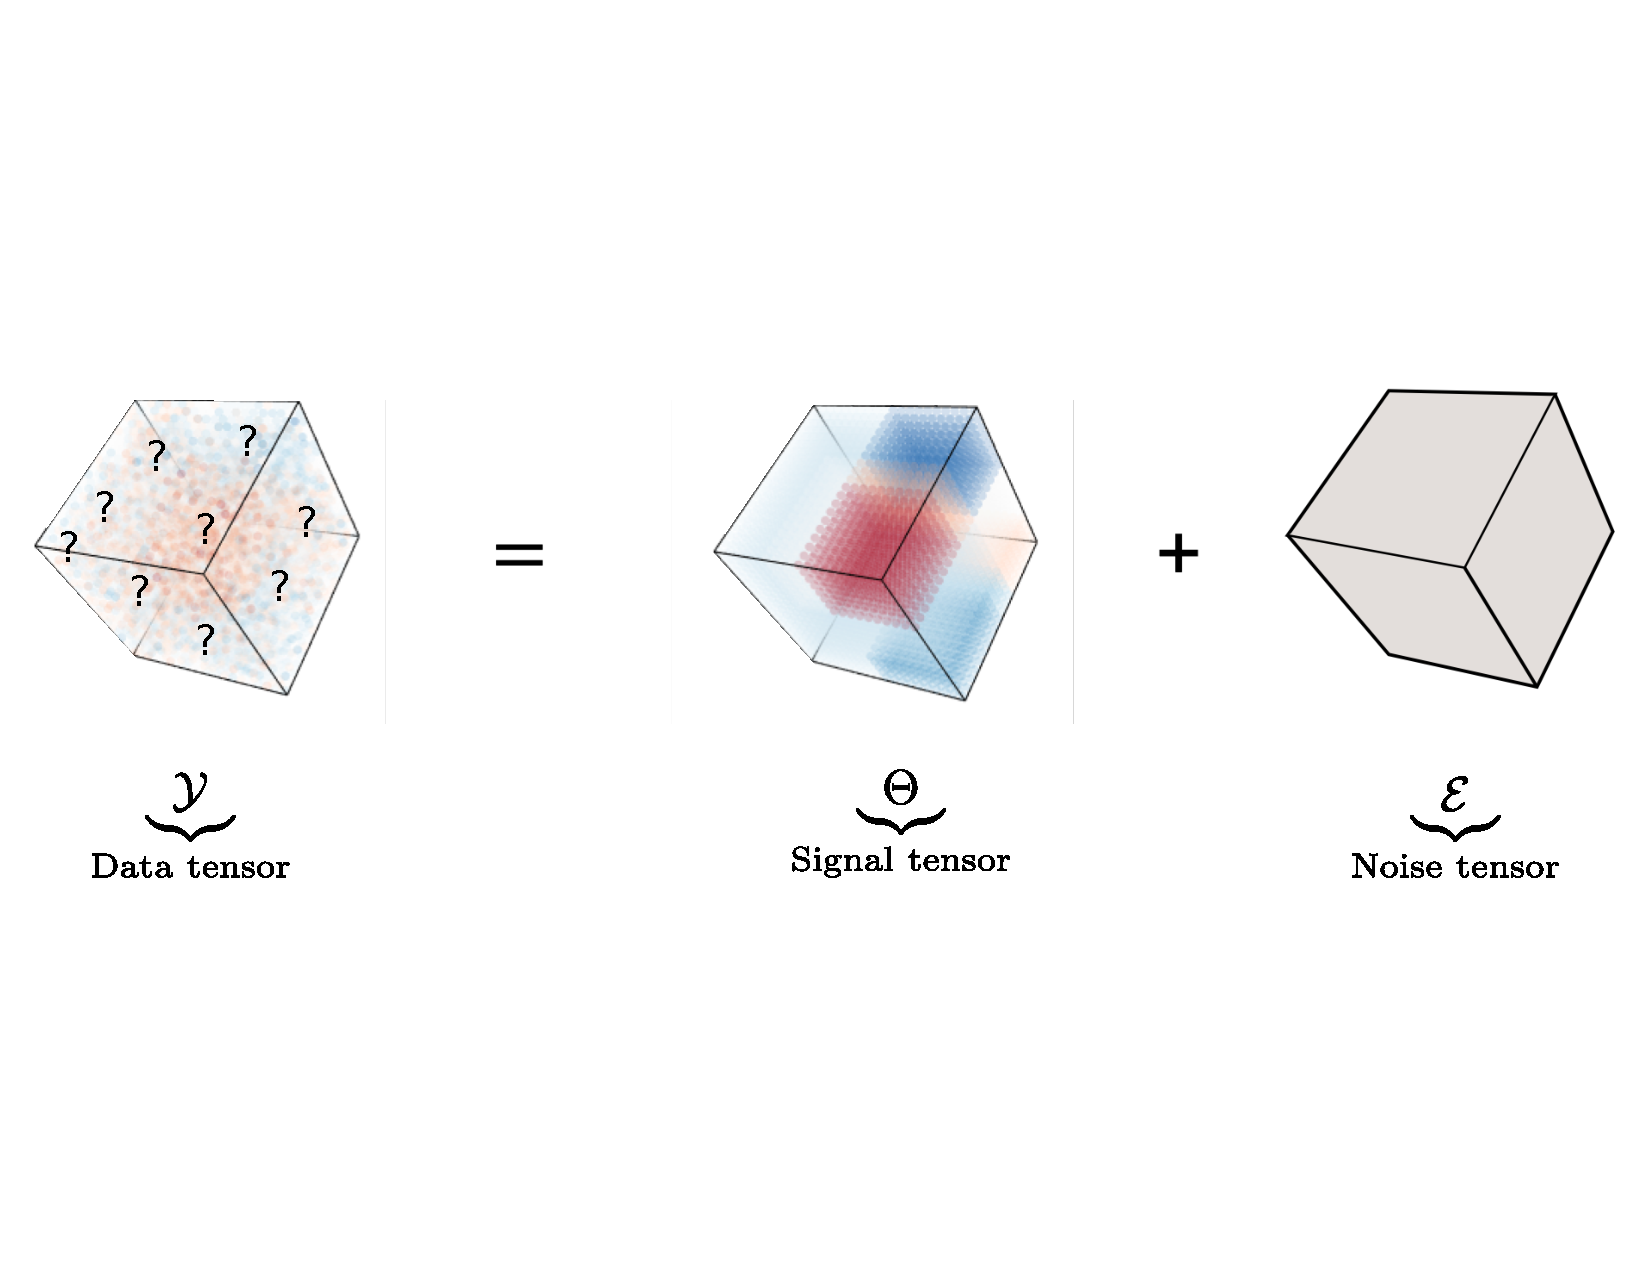
\includegraphics[width =\textwidth]{Figures/signalnoise.pdf}
    \end{center}
  
\end{frame}


\begin{frame}{Sign rank}
\begin{itemize}
    \item Key ideas: we use {\color{red}a local (nonparametric) notion of ``low-rankness''} to allow a broad family of signal tensors. 
        
    \item  Two tensors are sign equivalent, denoted $\Theta \simeq \Theta'$, if $\text{sgn}(\Theta) = \text{sgn}(\Theta')$.

    \item Define the {\color{red}sign rank} by
  \begin{align}
    \rlap{\textcolor{blue!10}{\rule[-\dp\strutbox]{235pt}{\baselineskip}}}\,\text{srank}(\Theta) = \min\{\text{rank}(\Theta')\colon \Theta'\simeq \Theta, \ \Theta'\in\mathbb{R}^{d_1\times\cdots\times d_K}\}.
\end{align}
    
 \begin{center}
    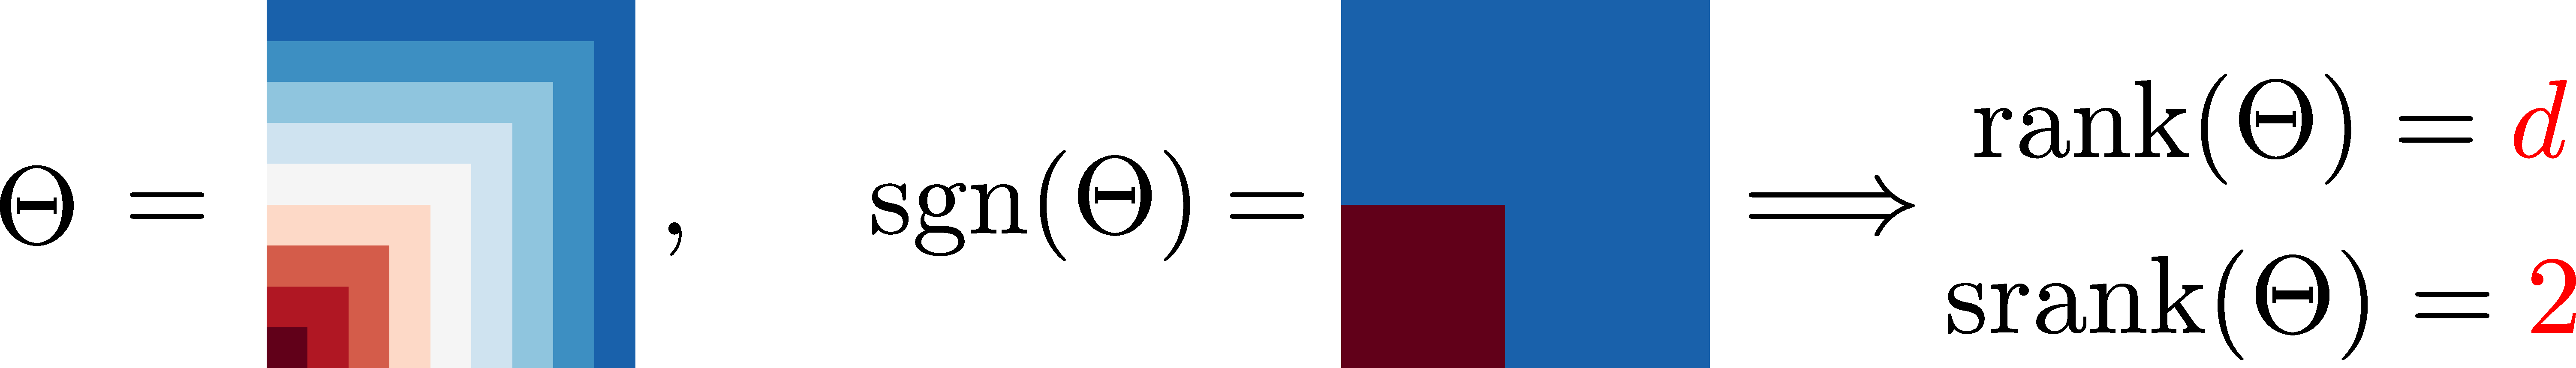
\includegraphics[width =.9\textwidth]{Figures/signrank_new.pdf}
    \end{center}
\item For any strictly monotonic function $g\colon\mathbb{R}\rightarrow \mathbb{R}$ with $g(0) = 0$,
\[\rlap{\textcolor{blue!10}{\rule[-\dp\strutbox]{105pt}{\baselineskip}}}\,\text{srank}(\Theta)\leq \text{rank}(g(\Theta)).\]
\end{itemize}
\end{frame}

\begin{frame}{Sign representable tensors}
    \begin{block}{Sign representable tensors} 
A tensor $\Theta$ is called {\color{red}$r$-sign representable} if the tensor $(\Theta-\pi)$ has sign rank bounded by $r$ for all $\pi\in[-1,1].$ 
    \end{block}
    \begin{itemize}
   \item Most existing structured tensors belong to sign representable family:
    \begin{itemize}
      \item {\color{red}Low-rank} CP tensors, Tucker tensors, stochastic tensor block models.
       \item {\color{red}High-rank} tensors from GLM, single index models. 
        \item Earlier example $\small \Theta(i_1,\ldots,i_K) = \log(1+\max(i_1,\ldots,i_K))$ is 2-sign representable $\Rightarrow$ properties extends to general max/min hypergraphon models. 
    \end{itemize} 
    
       \item We propose the signal tensor family
       \begin{align}
         \rlap{\textcolor{blue!10}{\rule[-\dp\strutbox]{250pt}{\baselineskip}}}\,  \Theta\in\caliP(r):=\{\Theta\colon\text{srank}(\Theta-\pi)\leq r \text{ for all } \pi\in[-1,1]\}.
       \end{align}
      \end{itemize}
\end{frame}


\begin{frame}{Our solution: sign signal helps!}
 
     \begin{center}
     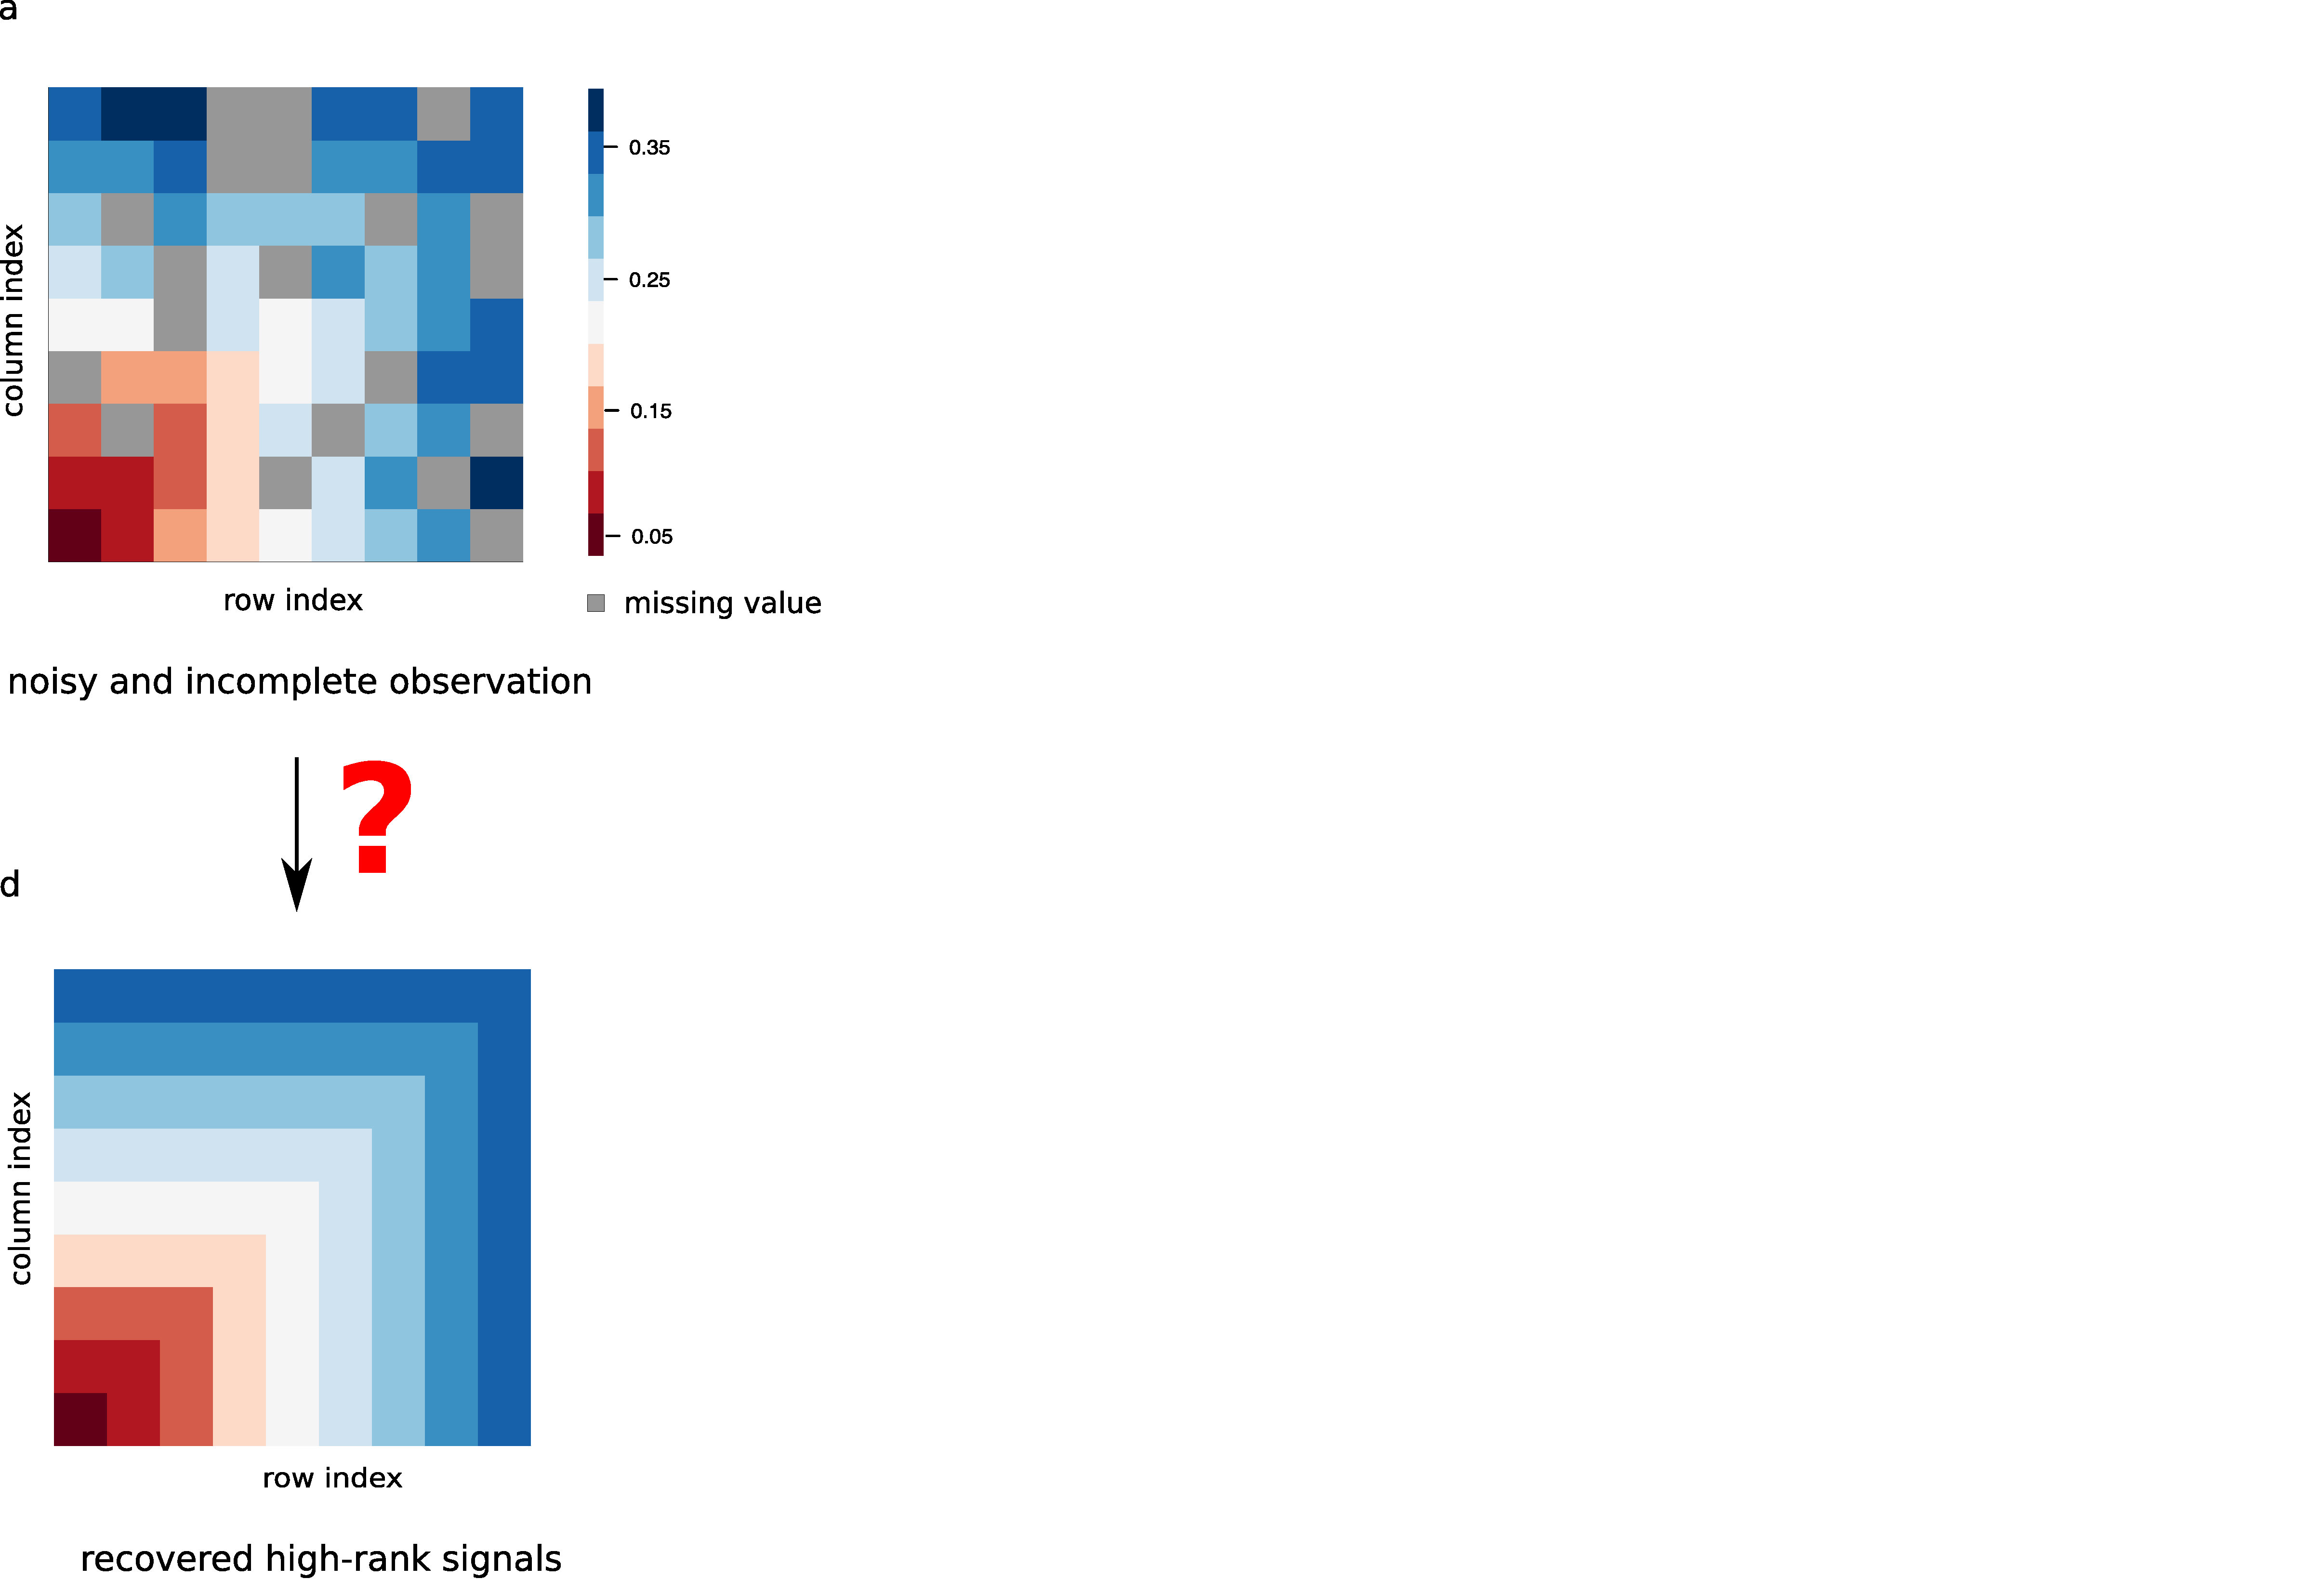
\includegraphics[width =\textwidth]{Figures/mainidea_step1.pdf}
        \end{center}
   \end{frame}

\begin{frame}{Our solution: sign signal helps!}
     \begin{center}
 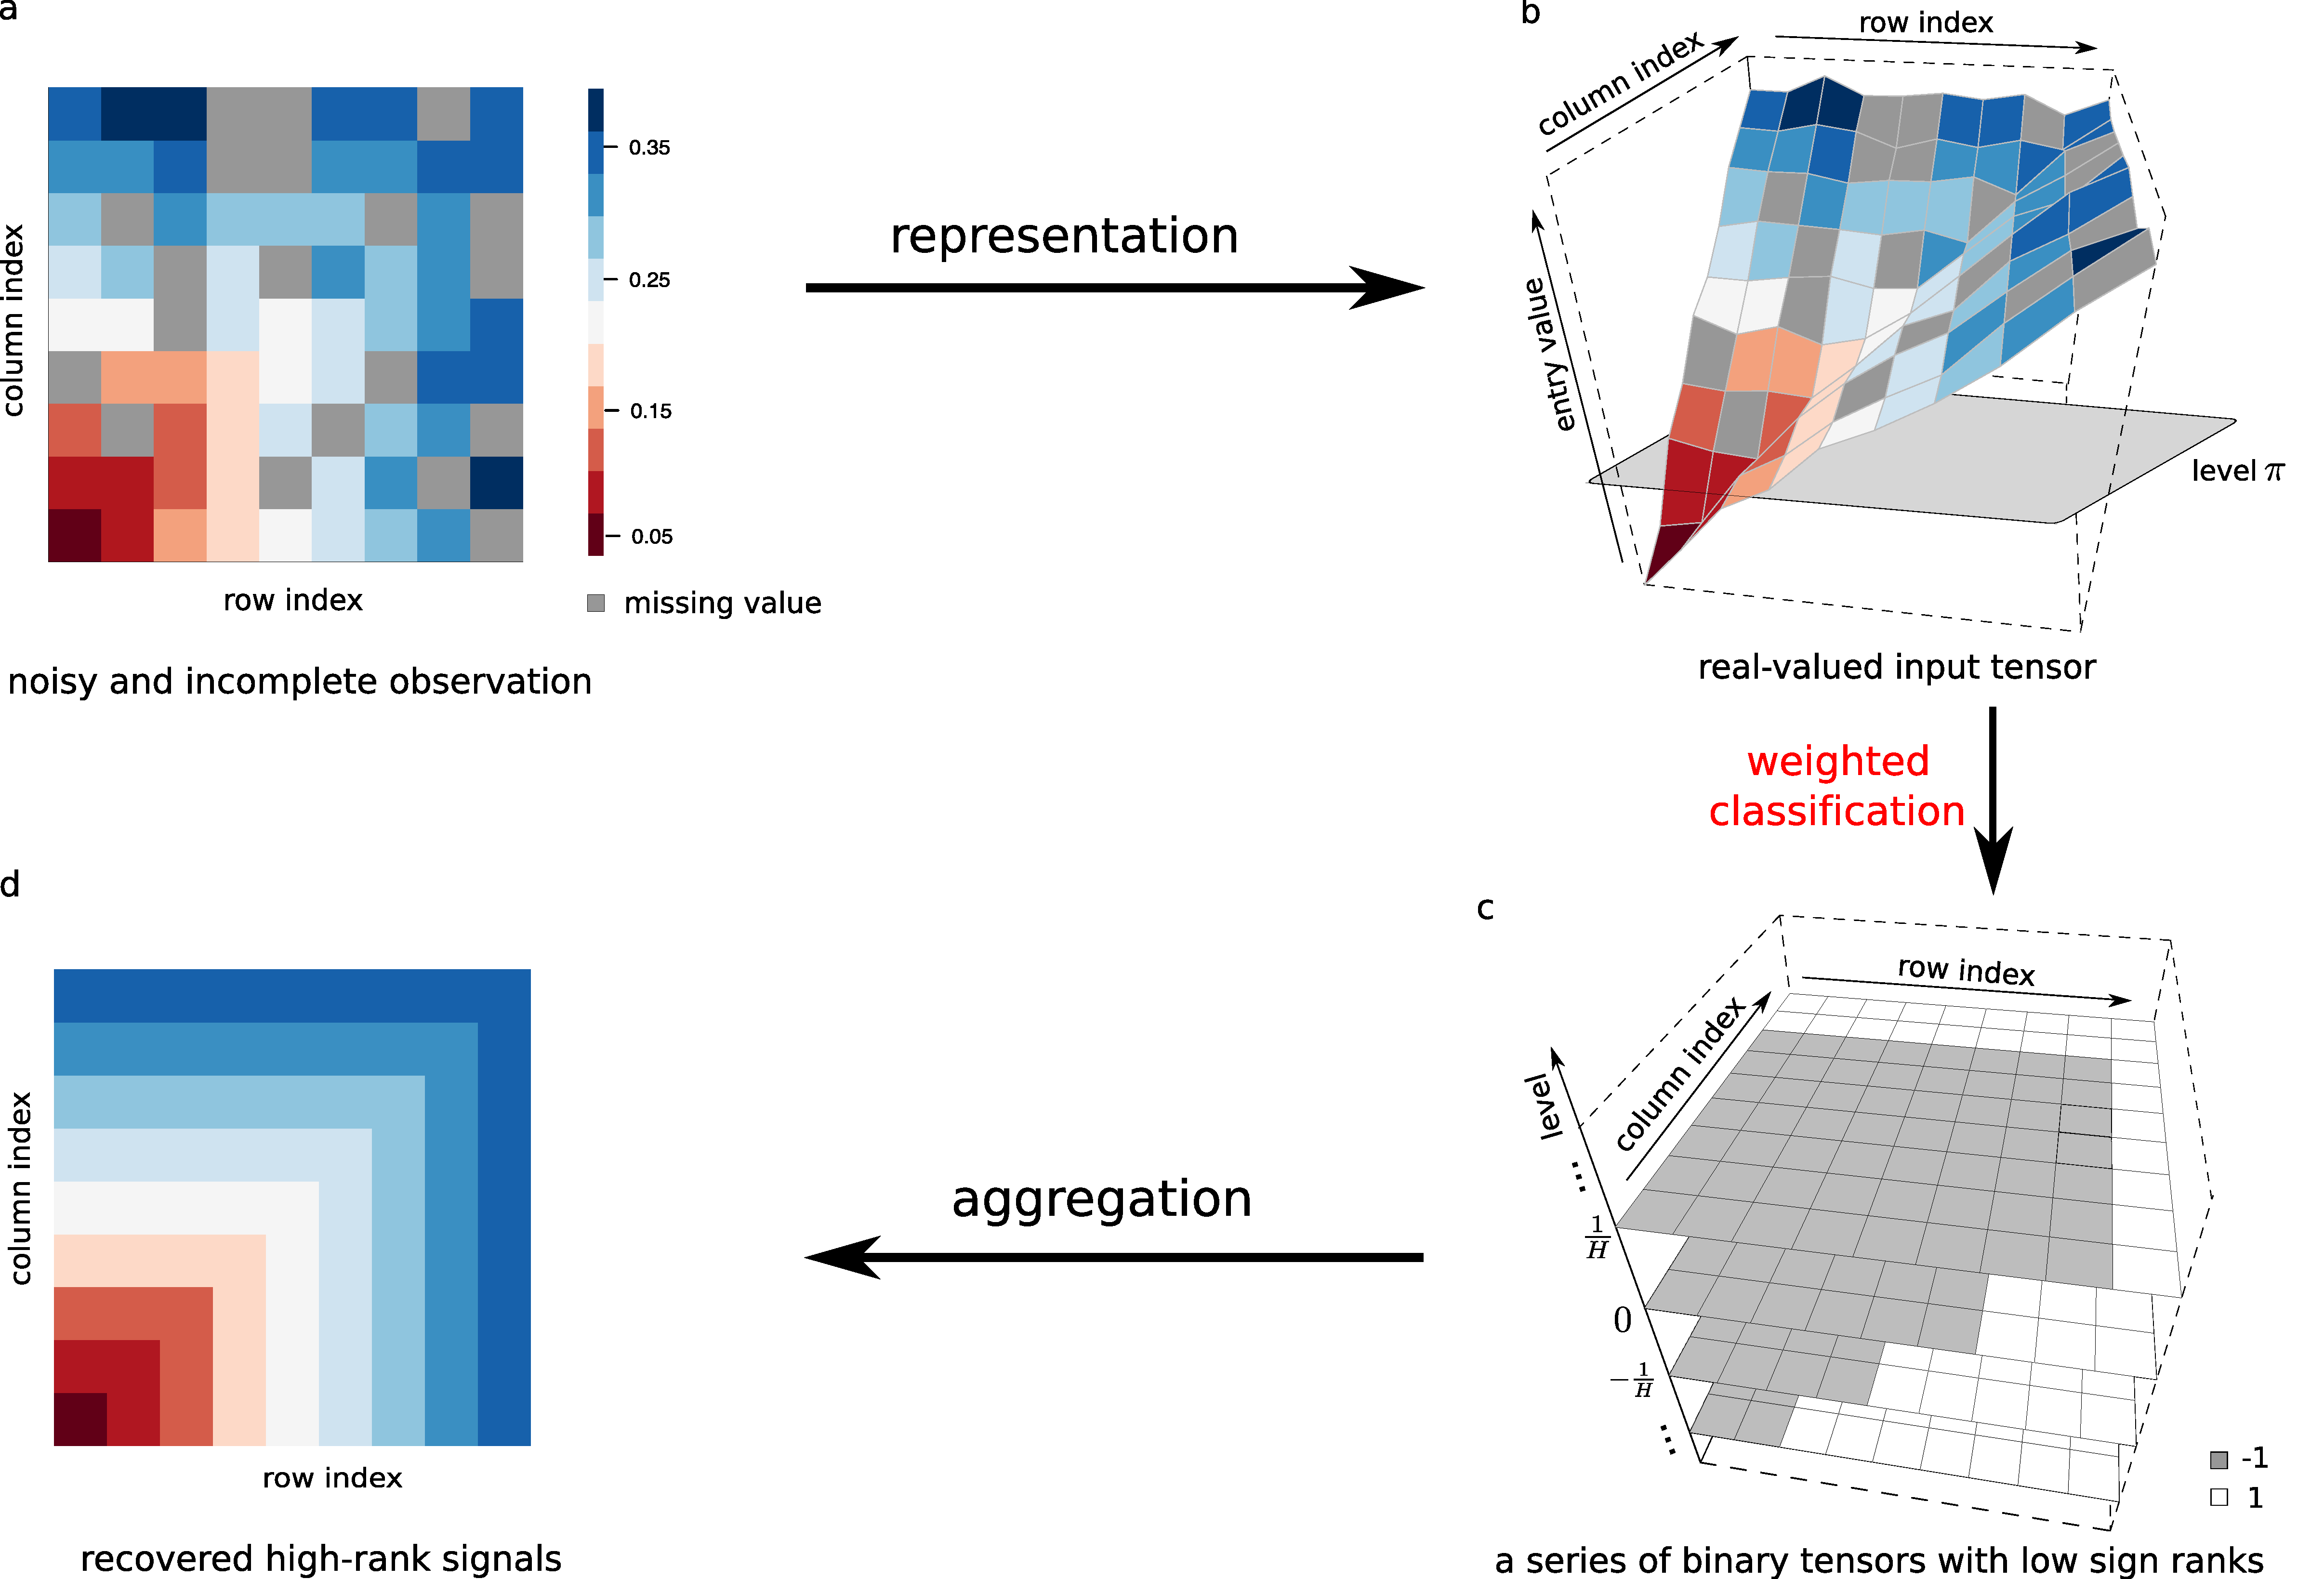
\includegraphics[width =\textwidth]{Figures/mainidea.pdf}
         \end{center}
 \end{frame}

\begin{frame}{Sign representation}
\begin{itemize}
    \item We observe {\color{red}a noisy incomplete tensor} $\tY_\Omega\in[-1,1]^{d_1\times \cdots\times d_K}$ with observed index set $\Omega\in[d_1]\times\cdots\times[d_K]$ under uniform sampling scheme. 
    \item We dichotomize the data into {\color{red}a series of sign tensors}:
\[
\{\sign(\tY_\Omega-\pi)\}_{\pi\in \tH}, \quad \text{where}\ \tH=\left\{-1,\ldots, -{1\over H}, 0, {1\over H}, \ldots, 1\right\}. 
\]
\end{itemize}
        
  \begin{center}
    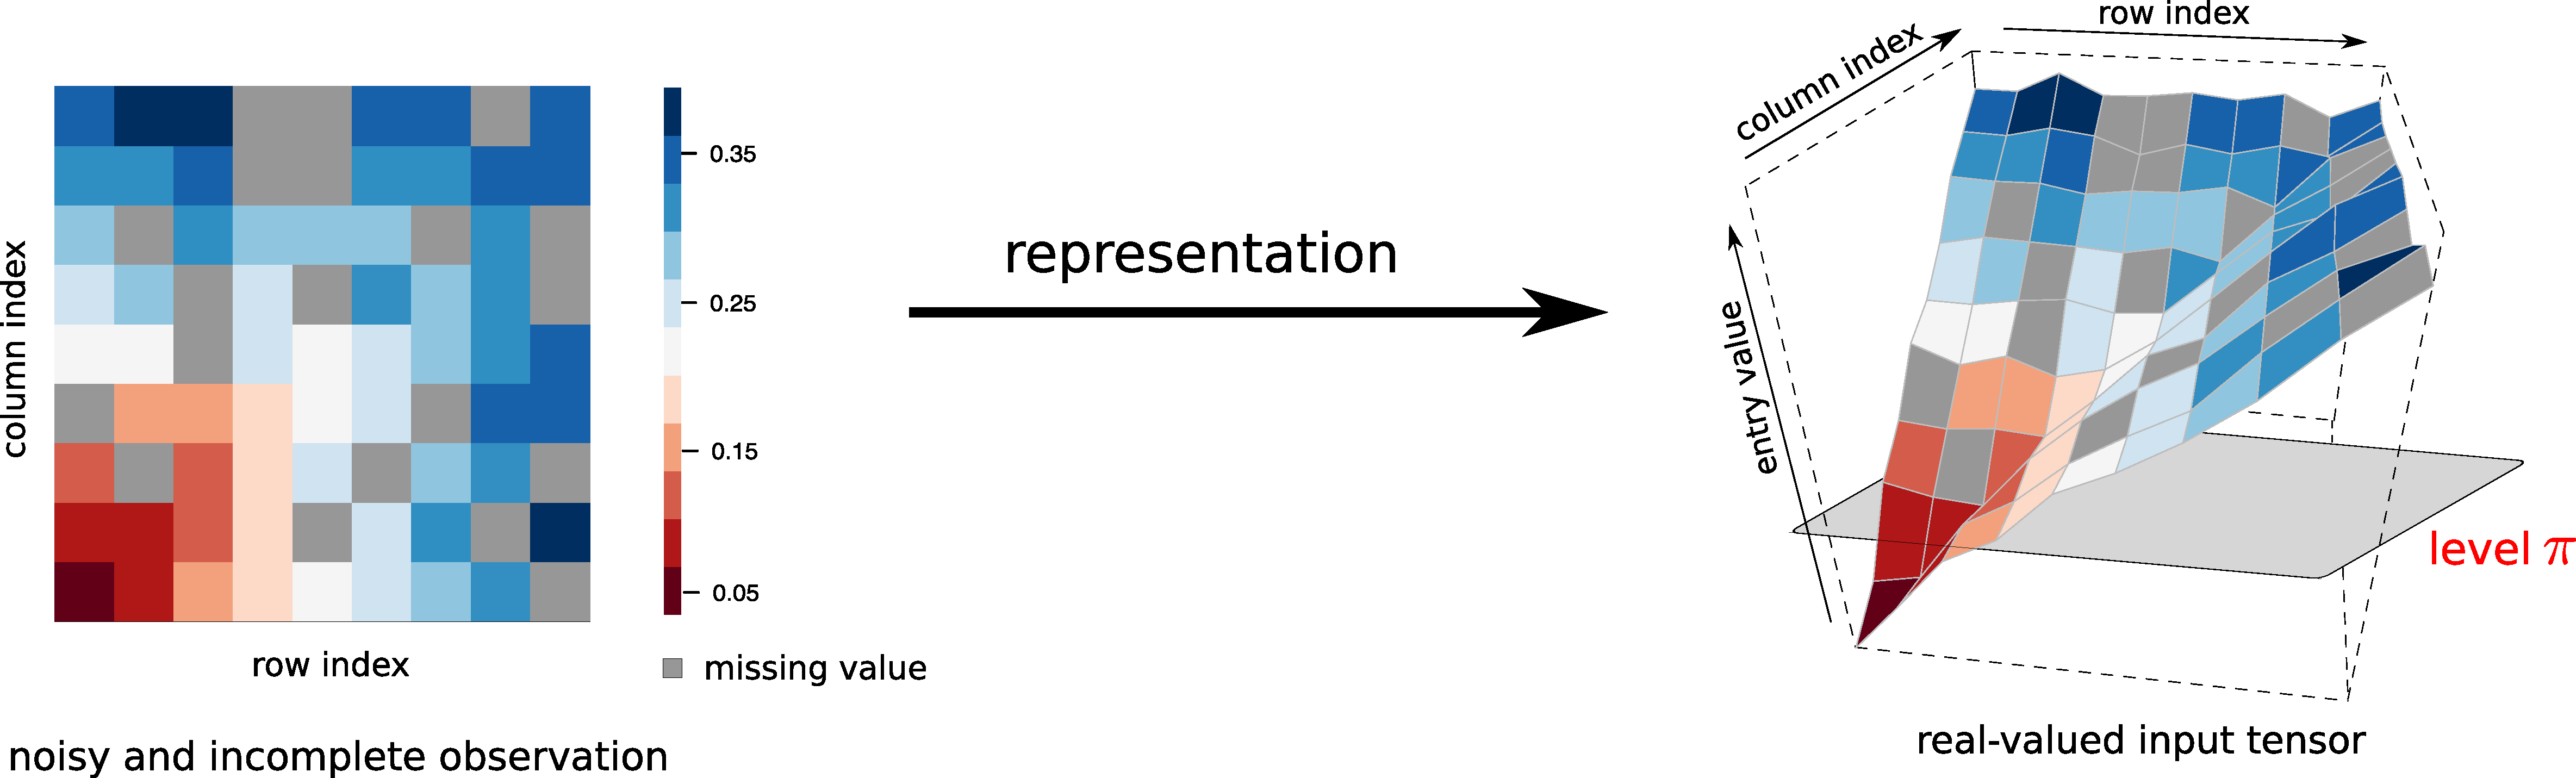
\includegraphics[width =\textwidth]{Figures/representation.pdf}
    \end{center}
\end{frame}

\begin{frame}{Sign estimation via weighted classification}
    \begin{itemize}
    \item We estimate {\color{red}$\text{sgn}(\Theta-\pi)$} through {\color{red}$\text{sgn}(\tY_\Omega-\pi)$} via weighted classification.
    \item Objective function of weighted classification is
    \begin{align}
    L({\color{red}\tZ},\tY_\Omega-\pi) = \frac{1}{|\Omega|}\sum_{\pi\in\Omega}\underbrace{|\tY(\omega)-\pi|}_{\text{weight}}\times\underbrace{ |{\color{red}\text{sgn}(\tZ(\omega))}-\text{sgn}(\tY(\omega)-\pi)|}_{\text{classification loss}}
    \end{align}
    \end{itemize}
      \begin{center}
    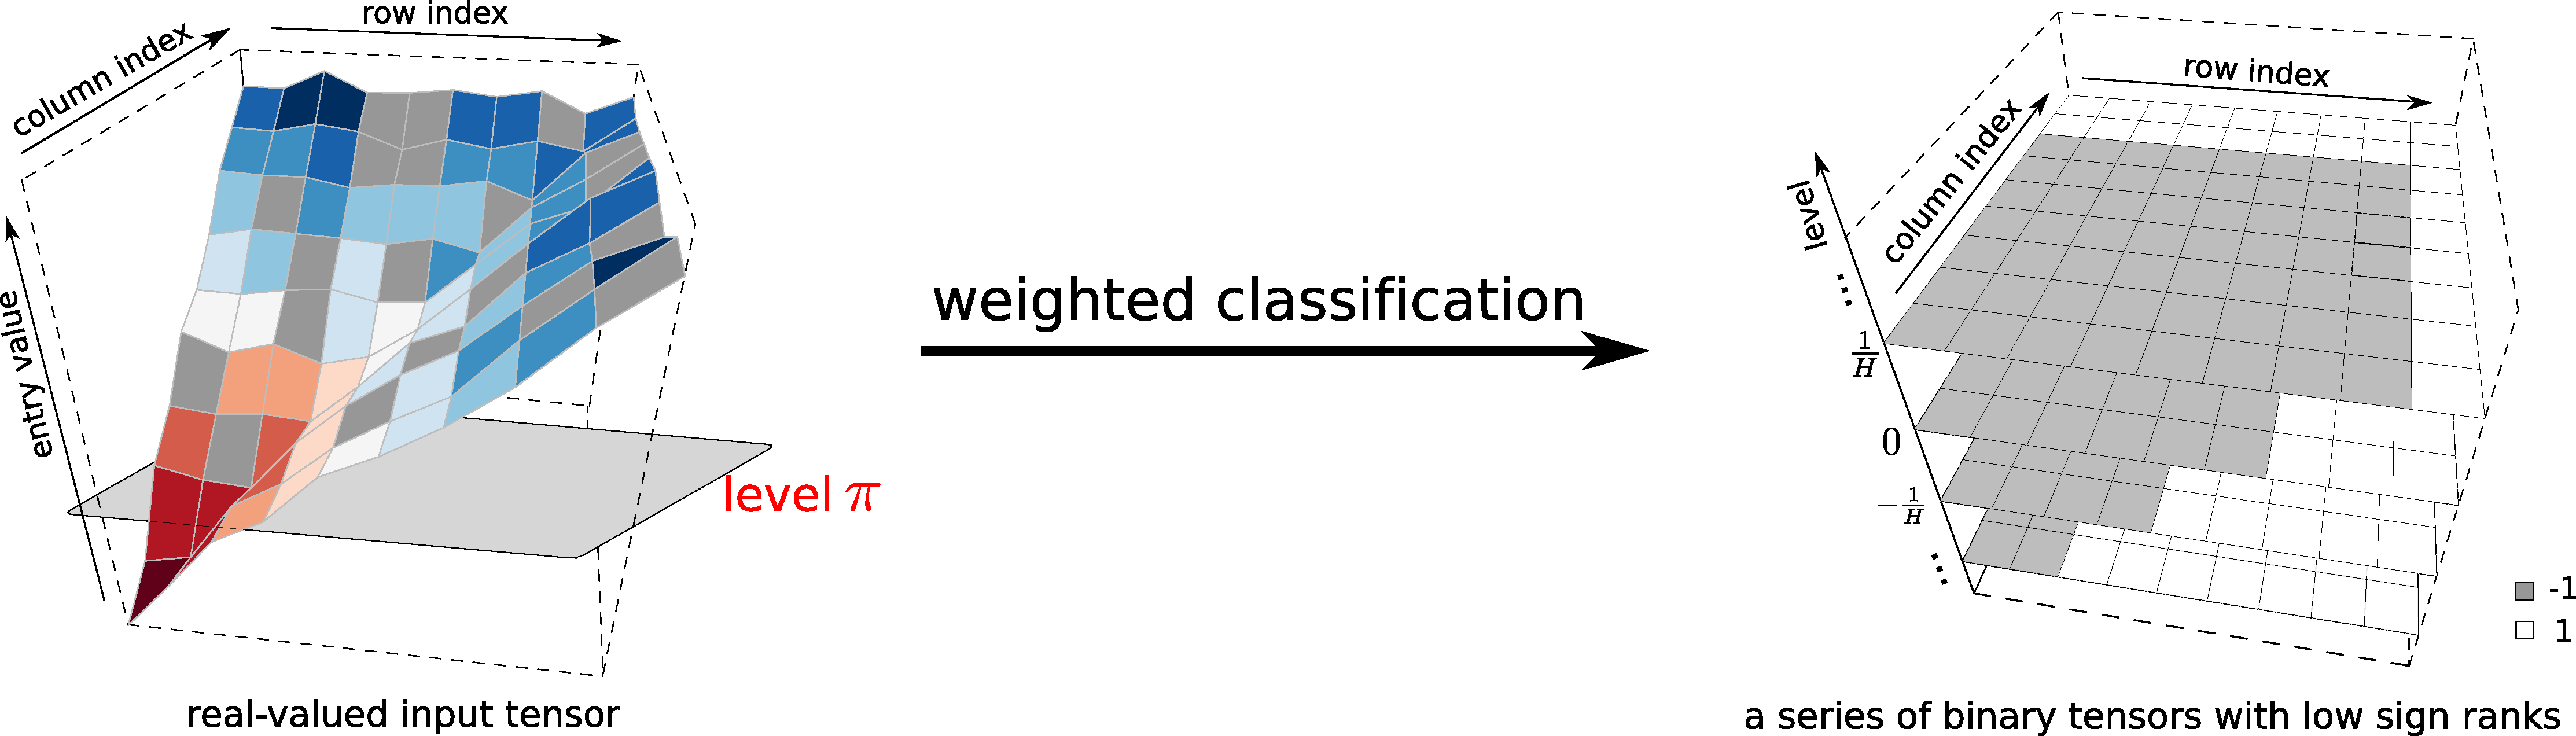
\includegraphics[width =\textwidth]{Figures/weightedclassification.pdf}
    \end{center}
    
\end{frame}


\begin{frame}{Identification for sign tensor estimation}
\begin{block}{$\alpha$-smoothness of signal tensor}
For fixed $\pi$, $\Theta$ is $\alpha$-smooth if there exist $\alpha = \alpha(\pi)>0,c = c(\pi)>0$, s.t.
\begin{align}
    \sup_{0\leq t<\rho(\pi,\tN)}{\mathbb{P}_{\omega\sim\Pi}[|{\color{red}\Theta(\omega)-\pi}|\leq {\color{blue}t}]\over {\color{blue}t^\alpha}}\leq c,
\end{align}
where $\rho(\pi,\tN) = \min_{\pi'\in\tN}|\pi-\pi'|$ and $\tN = \{\pi\colon\mathbb{P}(\Theta(\omega) = \pi)\neq 0\}$.
If $\alpha$ and $c$ are global constants for all$^*$ $\pi$'s, we call $\Theta$ is $\alpha$-globally smooth.
\end{block}
 \vspace{-.4cm}
 {\hfill \tiny $^*$ except for a finite number of $\pi$'s. }
 \vspace{-.2cm} 
 
 \pause
Intuition: {\color{red}sign recovery} is harder at {\color{red}levels where point mass concentrates}. 
Rate depends on the behavior of CDF function $G(\pi)=\mathbb{P}_{\omega\sim \Pi}[\Theta(\omega)\leq \pi]$. 
 \begin{center}
 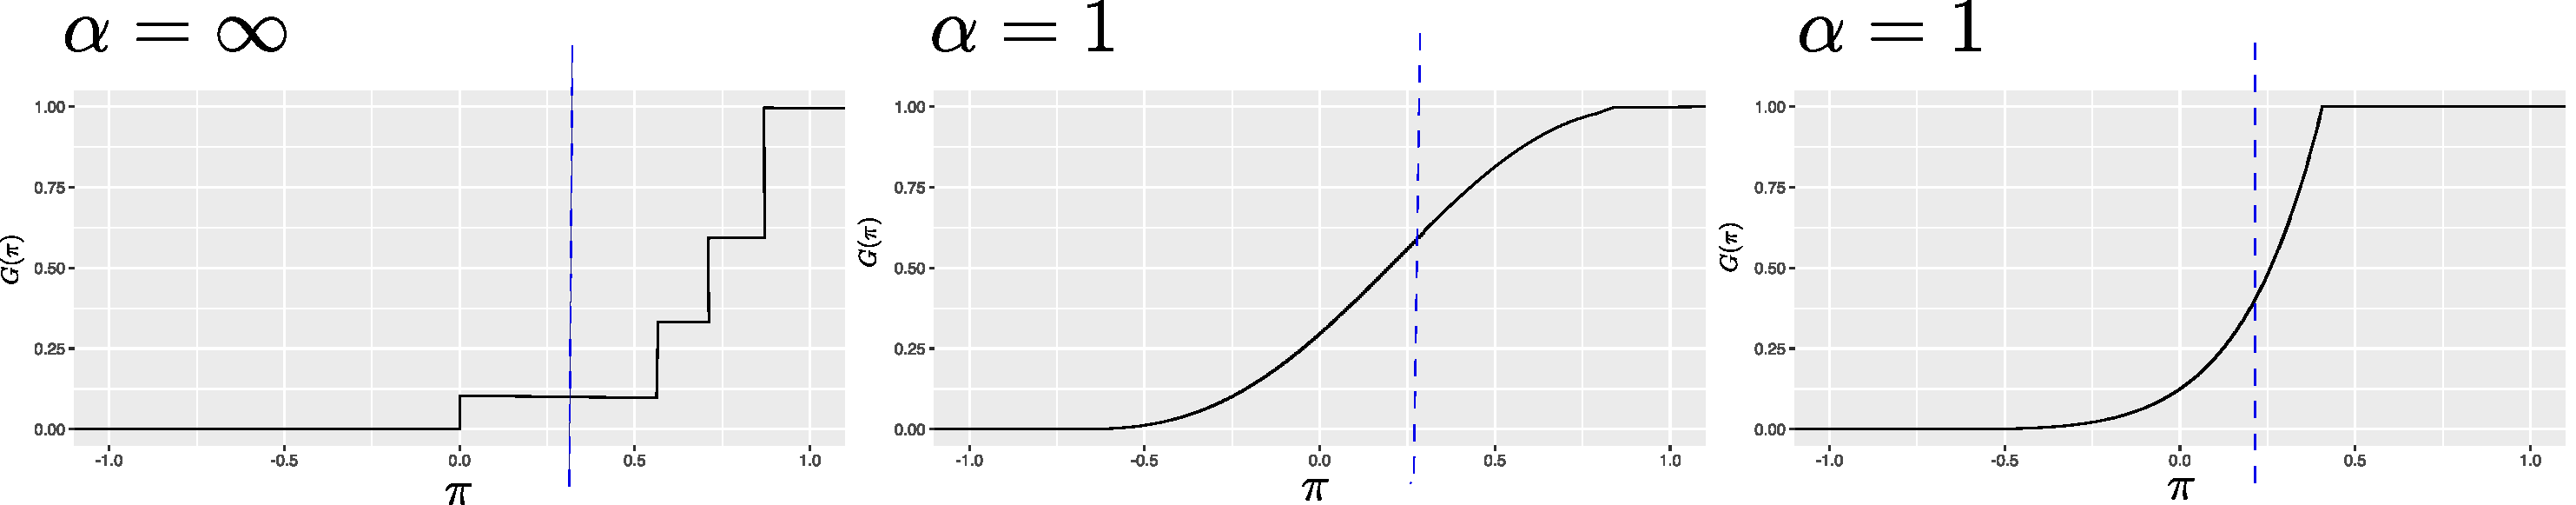
\includegraphics[width = \textwidth]{Figures/cdf_new.pdf}
 \end{center}
\end{frame}

\begin{frame}{Identification for sign tensor estimation}
   \begin{itemize}
    \item If $\Theta$ is $\alpha$-smooth ($\alpha>0$), we have {\color{red}a unique optimizer}  such that\\[.1cm]
       $\hspace{2cm}\text{sgn}(\Theta-\pi) = \argmin\limits_{\tZ\colon \text{rank}(\tZ)\leq r} \mathbb{E}_{\tY_\Omega}L(\tZ,\tY_\Omega-\pi)$.\vspace*{.1cm}

    \item We obtain a series of optimizers $\{\hat \tZ_\pi\}_{\pi\in\tH}$ as
    \begin{align}
        \hat \tZ_\pi = \argmin_{\tZ\colon \text{rank}(\tZ)\leq r}L(\tZ,\tY_\Omega-\pi).
    \end{align}
    \end{itemize}
 \vspace{-.2cm} 
 
     \begin{center}
 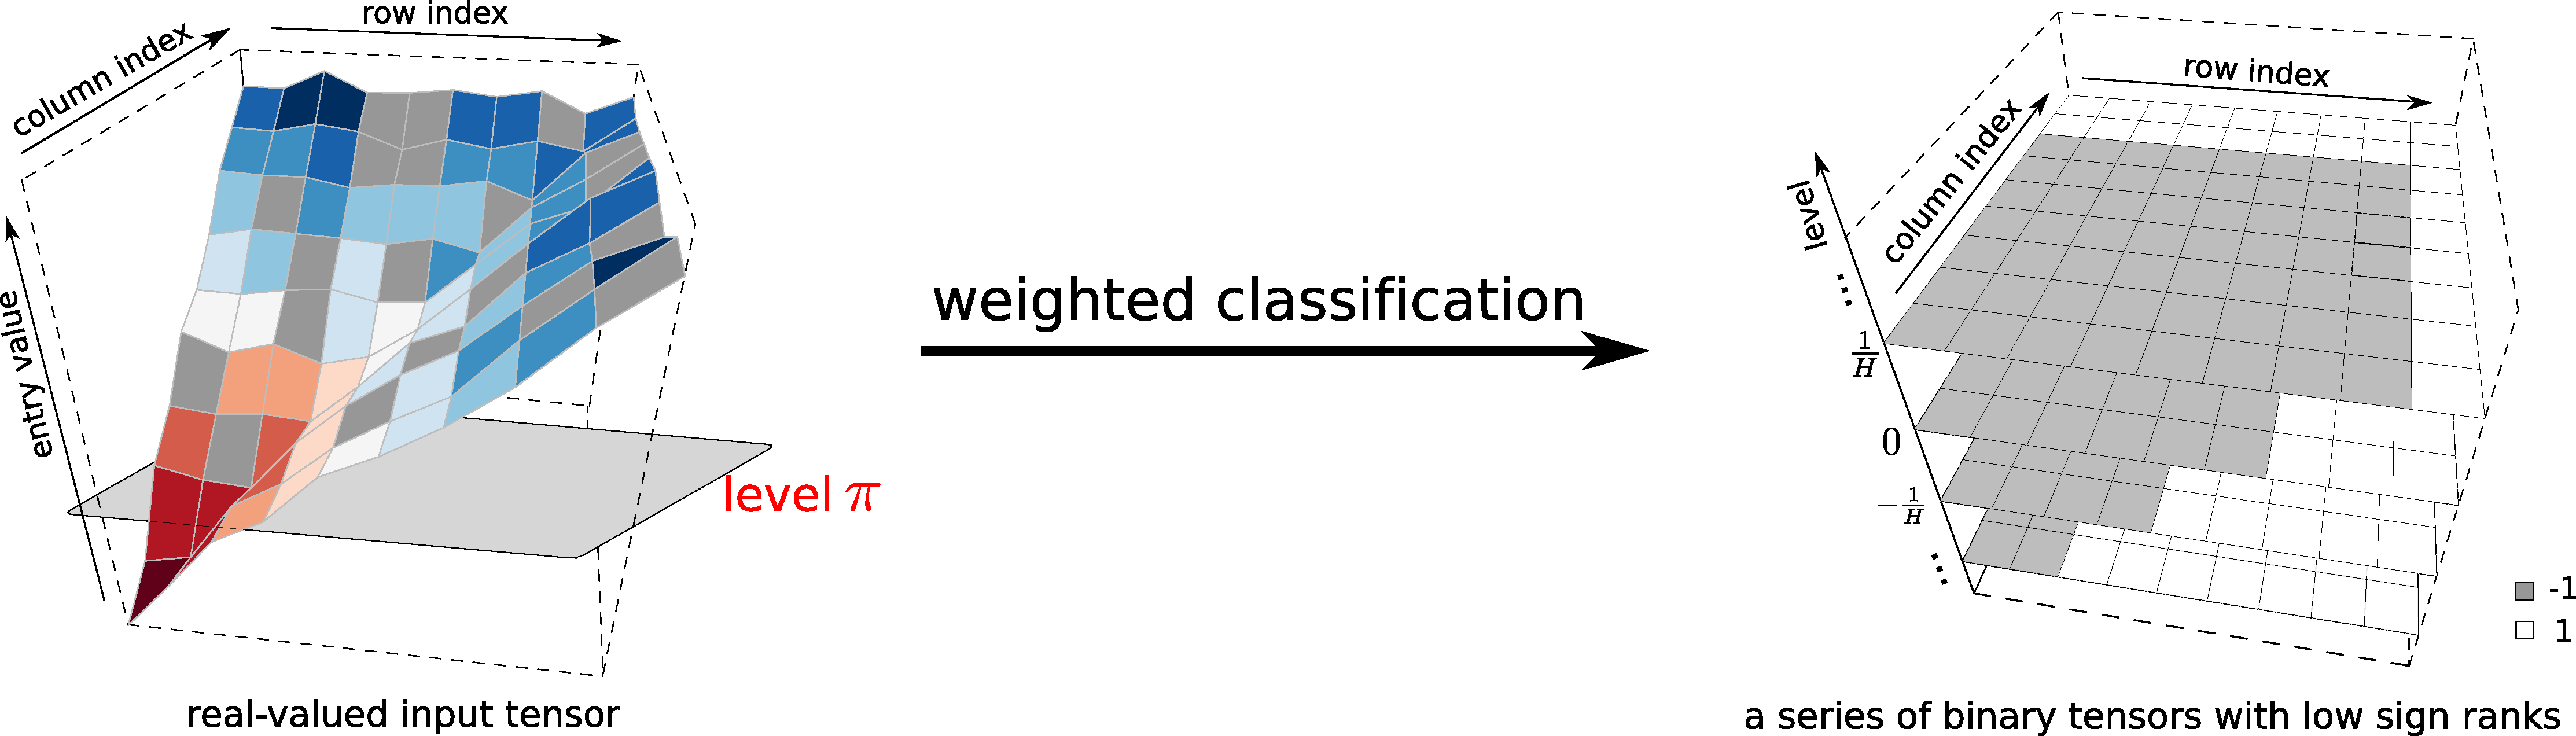
\includegraphics[width = \textwidth]{Figures/weightedclassification.pdf}
 \end{center}
 
     
     \vspace{-.4cm}
 {\hfill \tiny  $^*$Uniqueness up to sign equivalence, meaning the optimizer $\Theta_{\text{opt}} \simeq \sign(\Theta-\pi)$.}
\end{frame}


\begin{frame}{Sign tensor estimation error}
\begin{itemize}
\item For two tensor $\Theta_1,\Theta_2$, define $\textup{MAE}(\Theta_1,\Theta_2) = \mathbb{E}_{\omega\in\Pi}|\Theta_1(\omega)-\Theta_2(\omega)|.$
\end{itemize}
    \begin{block}{Sign tensor estimation for fixed $\pi$ (Lee and W. 2021)}
    Suppose $\Theta\in\caliP(r)$ and  $\Theta(\omega)$ is $\alpha$-smooth for fixed $\pi$. Let $d_{\max}=\max_{k\in[K]} d_k$. Then, with very high probability over $\tY_\Omega$, 
\begin{align}
\textup{MAE}(\text{sgn}\hat \tZ_\pi, \text{sgn}(\Theta-\pi)) \lesssim  \left({d_{\max} r\over |\Omega|}\right)^{\color{red}\alpha\over \alpha+2}.
\end{align}
    \end{block}
    \begin{itemize}
    \item Sign estimation error shows a polynomial decay with $|\Omega|$. 
    \item Best rate attains at $\alpha=\infty$ for stochastic tensor block models. 
    \end{itemize}
\end{frame}

\begin{frame}{From sign to signal estimation}
  
    \begin{itemize}
    \item Aggregation of sign tensors from weighted classification yields our signal tensor estimate:
    \begin{align}
        \hat\Theta = {1\over 2H+1}\sum_{\pi\in\tH}\text{sgn}\hat \tZ_\pi.
    \end{align}
    \vspace{-.5cm}
        \begin{center}
    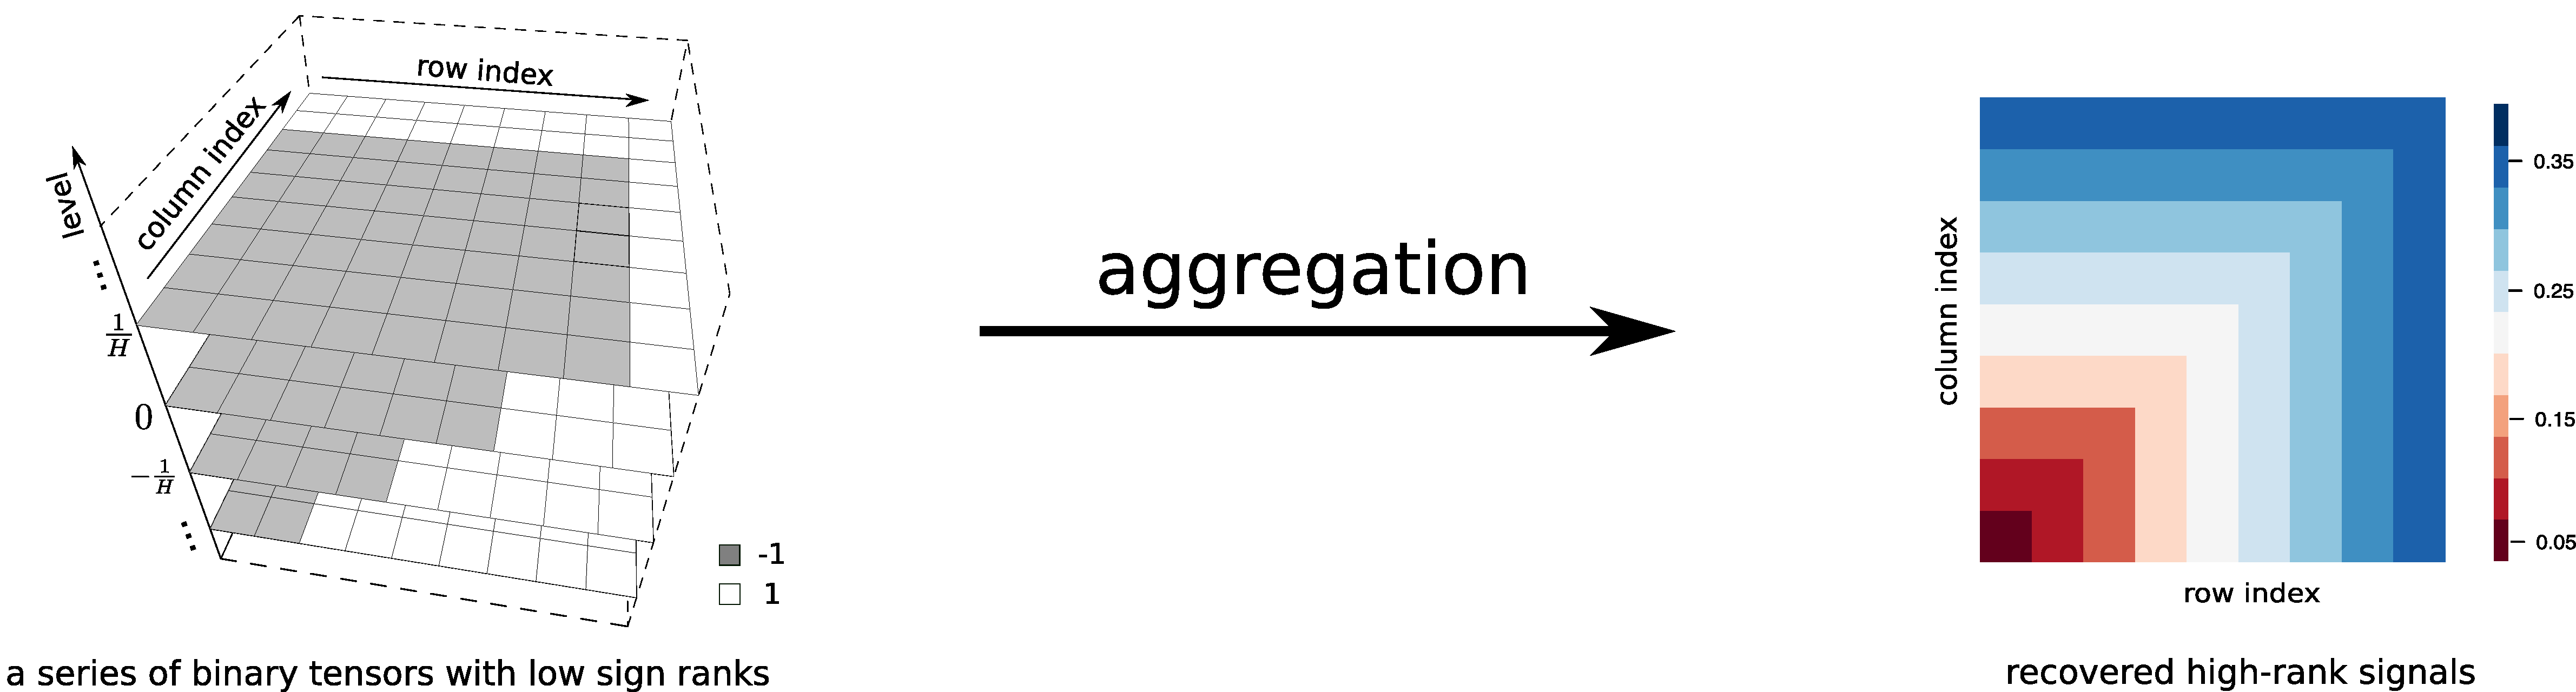
\includegraphics[width = .9\textwidth]{Figures/aggregation.pdf}
    \end{center}
    \item Signal tensor estimation is robust to a few off-target classifications. 
    
        \begin{center}
    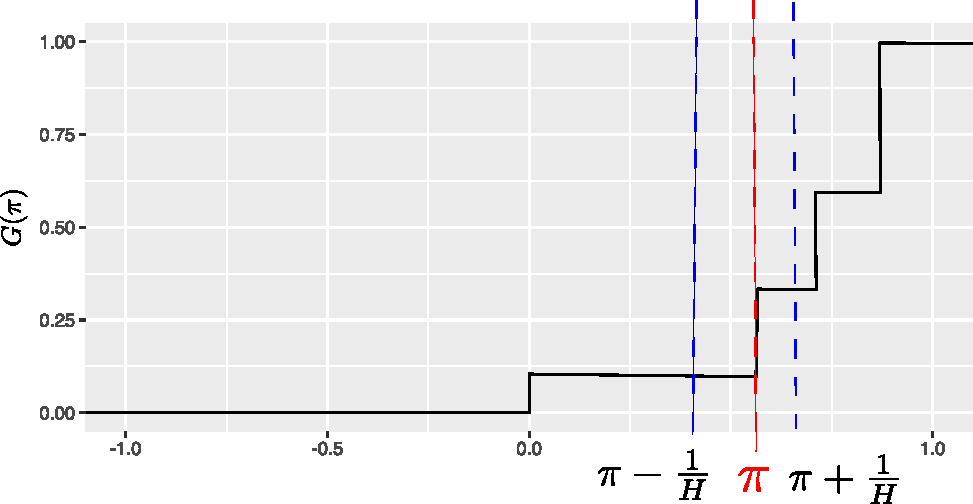
\includegraphics[width =.4\textwidth]{Figures/cdf_new_ave.pdf}
    \end{center}
    
    \end{itemize}

\end{frame}




\begin{frame}{Signal tensor estimation error}
    \begin{block}{Tensor estimation error (Lee and W. 2021)}
    Suppose $\Theta\in\caliP(r)$ and  $\Theta(\omega)$ is $\alpha$-globally smooth. Then, with very high probability over $\tY_\Omega$, 
    \begin{equation}\label{eq:bound2}
\textup{MAE}(\hat \Theta, \Theta)\lesssim \KeepStyleUnderBrace{\left({d_{\max} r \over |\Omega|}\right)^{\alpha\over\alpha+2}}_{\text{error inherited from sign estimation}}+\KeepStyleUnderBrace{{1\over \color{red}H}}_{\text{Bias}}+\KeepStyleUnderBrace{{{\color{red}H}d_{\max} r \over |\Omega|}}_{\text{Variance}}.
\end{equation}
In particular, setting $\scriptstyle H\asymp \left( |\Omega|\over d_{\max}r\right)^{1/2}$ yields the error bound
\begin{equation}\label{eq:real}
\textup{MAE}(\hat \Theta, \Theta)\lesssim \left(d_{\max}r \over |\Omega|\right)^{\color{red}{\alpha \over \alpha+2} \vee {1\over 2}}.
\end{equation}
    \end{block}
    \begin{itemize}
        \item Sample requirement for tensor completion:
         \[\text{MAE}(\hat\Theta,\Theta)\rightarrow 0, \text{ as } {|\Omega|\over {\color{red}d_{\max}r}}\rightarrow\infty.\]
    \end{itemize}
\end{frame}


\begin{frame}{Comparison of estimation error versus dimension}

    \begin{itemize}
\item We simulate signal tensors under a wide range of complexity.    

       \begin{center}
        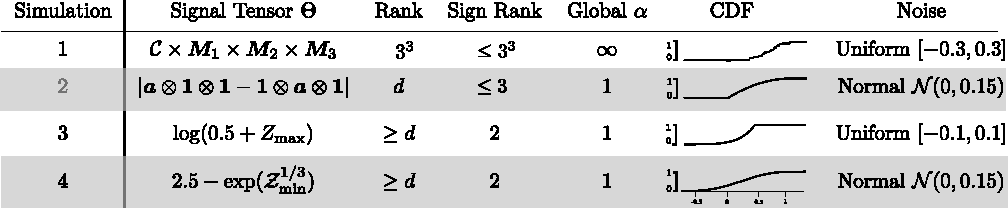
\includegraphics[width = \textwidth]{Figures/simulation_new.pdf}
        \end{center}

\pause
    \item Our method ({\color{blue}NonparaT}) achieves the best performance, whereas the second best method is low-rank CP tensor ({\color{red} CPT}) for models 1-2, and matrix nonparametric method ({\color{darkgreen} NonParaM}) for models 3-4.
  \end{itemize}
    
          \begin{center}
    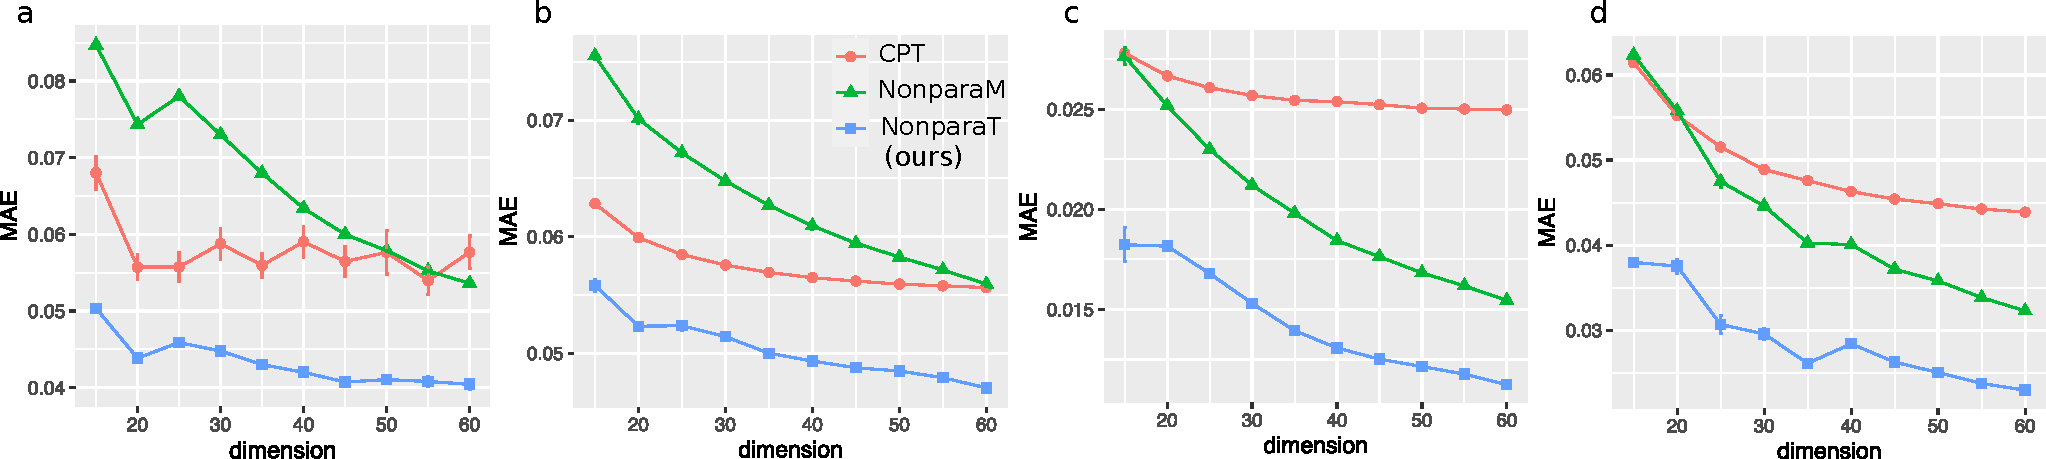
\includegraphics[width =\textwidth]{Figures/fig1-4v2.pdf}
    \end{center}
    
        
\end{frame}

\begin{frame}{Estimation error versus observation fraction}

    \begin{center}
        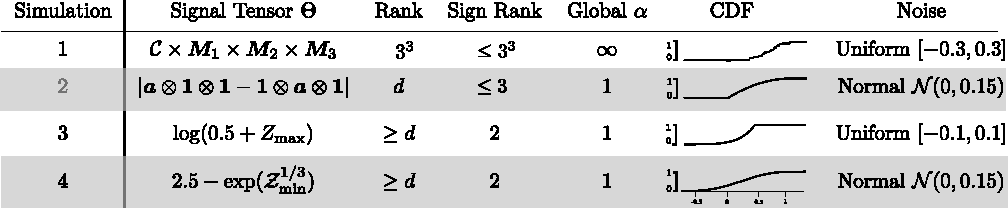
\includegraphics[width = \textwidth]{Figures/simulation_new.pdf}
        \end{center}
        
  \begin{itemize}
    \item Our method (NonparaT) achieves the best performance in completion. 
  \end{itemize}
    
    \begin{center}
  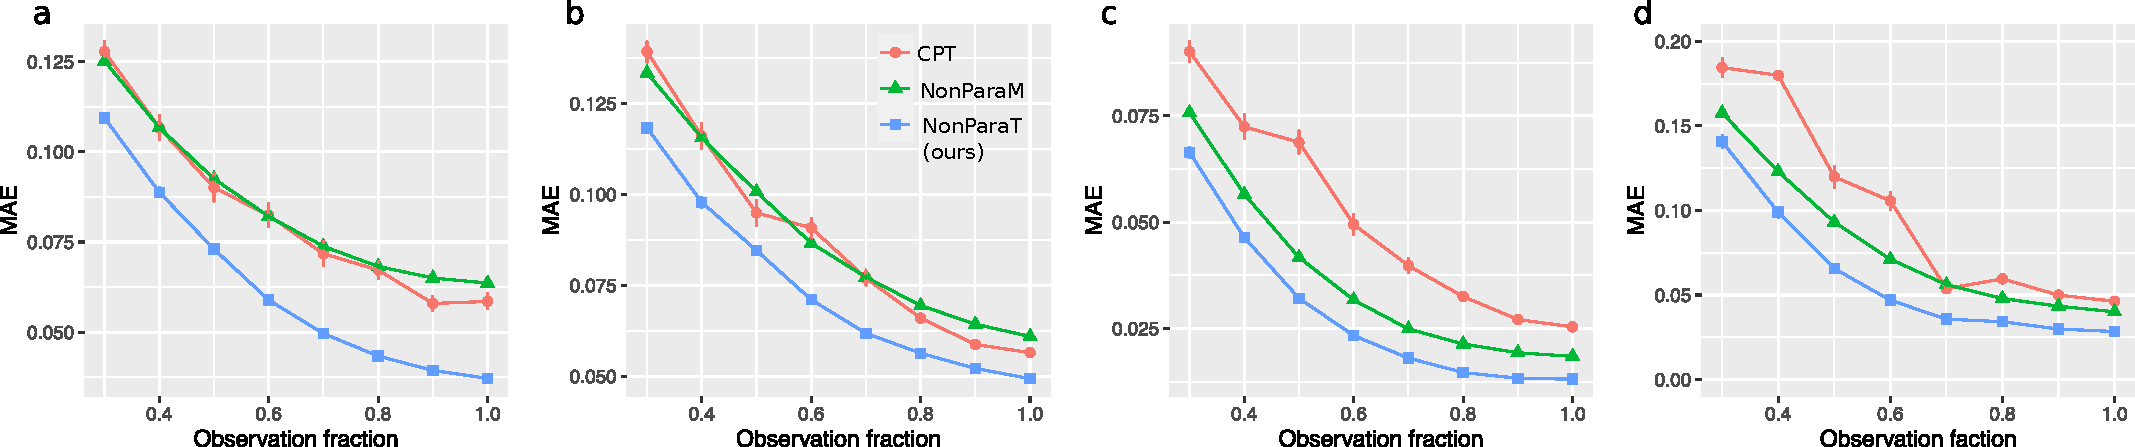
\includegraphics[width =\textwidth]{Figures/fig5-8v2.pdf}
  \end{center}
    
\end{frame}


\begin{frame}{Data application}

We apply our method to three datasets:
\begin{itemize}
\item The human brain connectivity data (Want et al '17) consists of 68 brain regions for 114 individuals along with their IQ scores.

\item The NIPS dataset (Globerson et al '07) consistis of word occurrence counts in papers published from 1987 to 2003.
\item The 3-channel image data is from licensed google image file.


\end{itemize}
    \begin{center}
    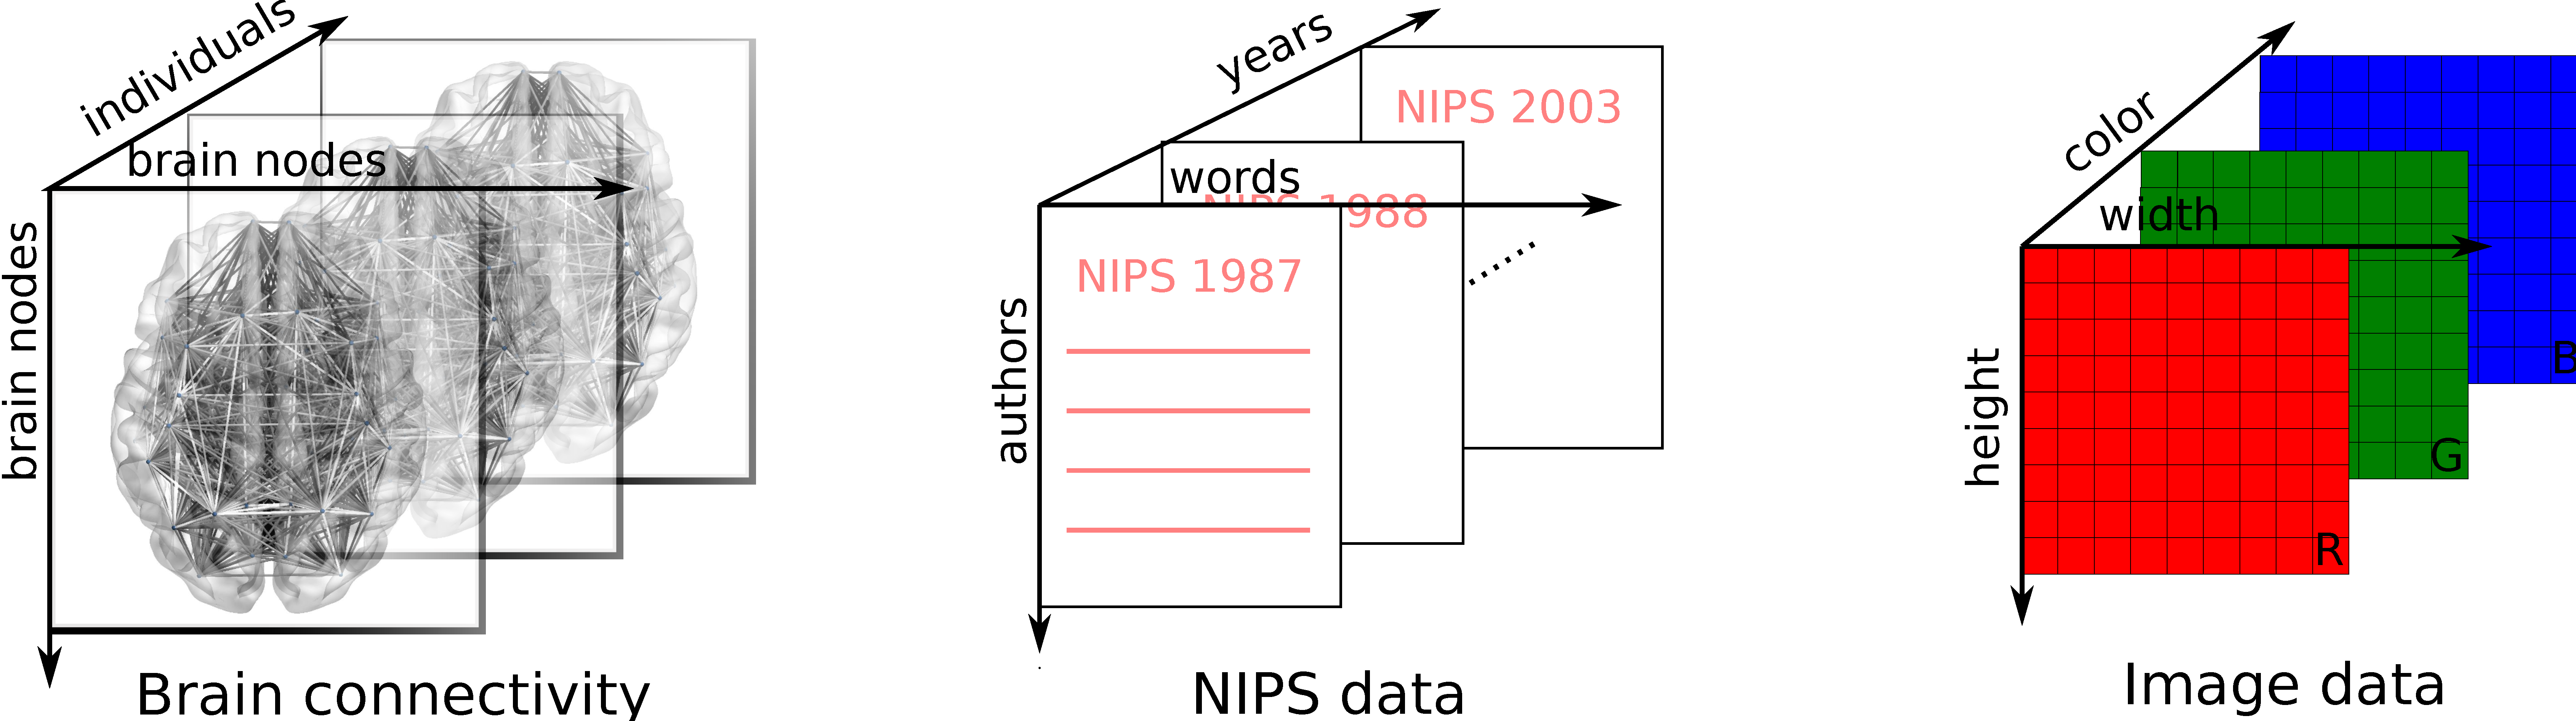
\includegraphics[width =\textwidth]{Figures/ndataset.pdf}
    \end{center}
\end{frame}

\begin{frame}{Data application: Brain connectivity}
\begin{columns}
\begin{column}{0.21\textwidth}
   \begin{center}
     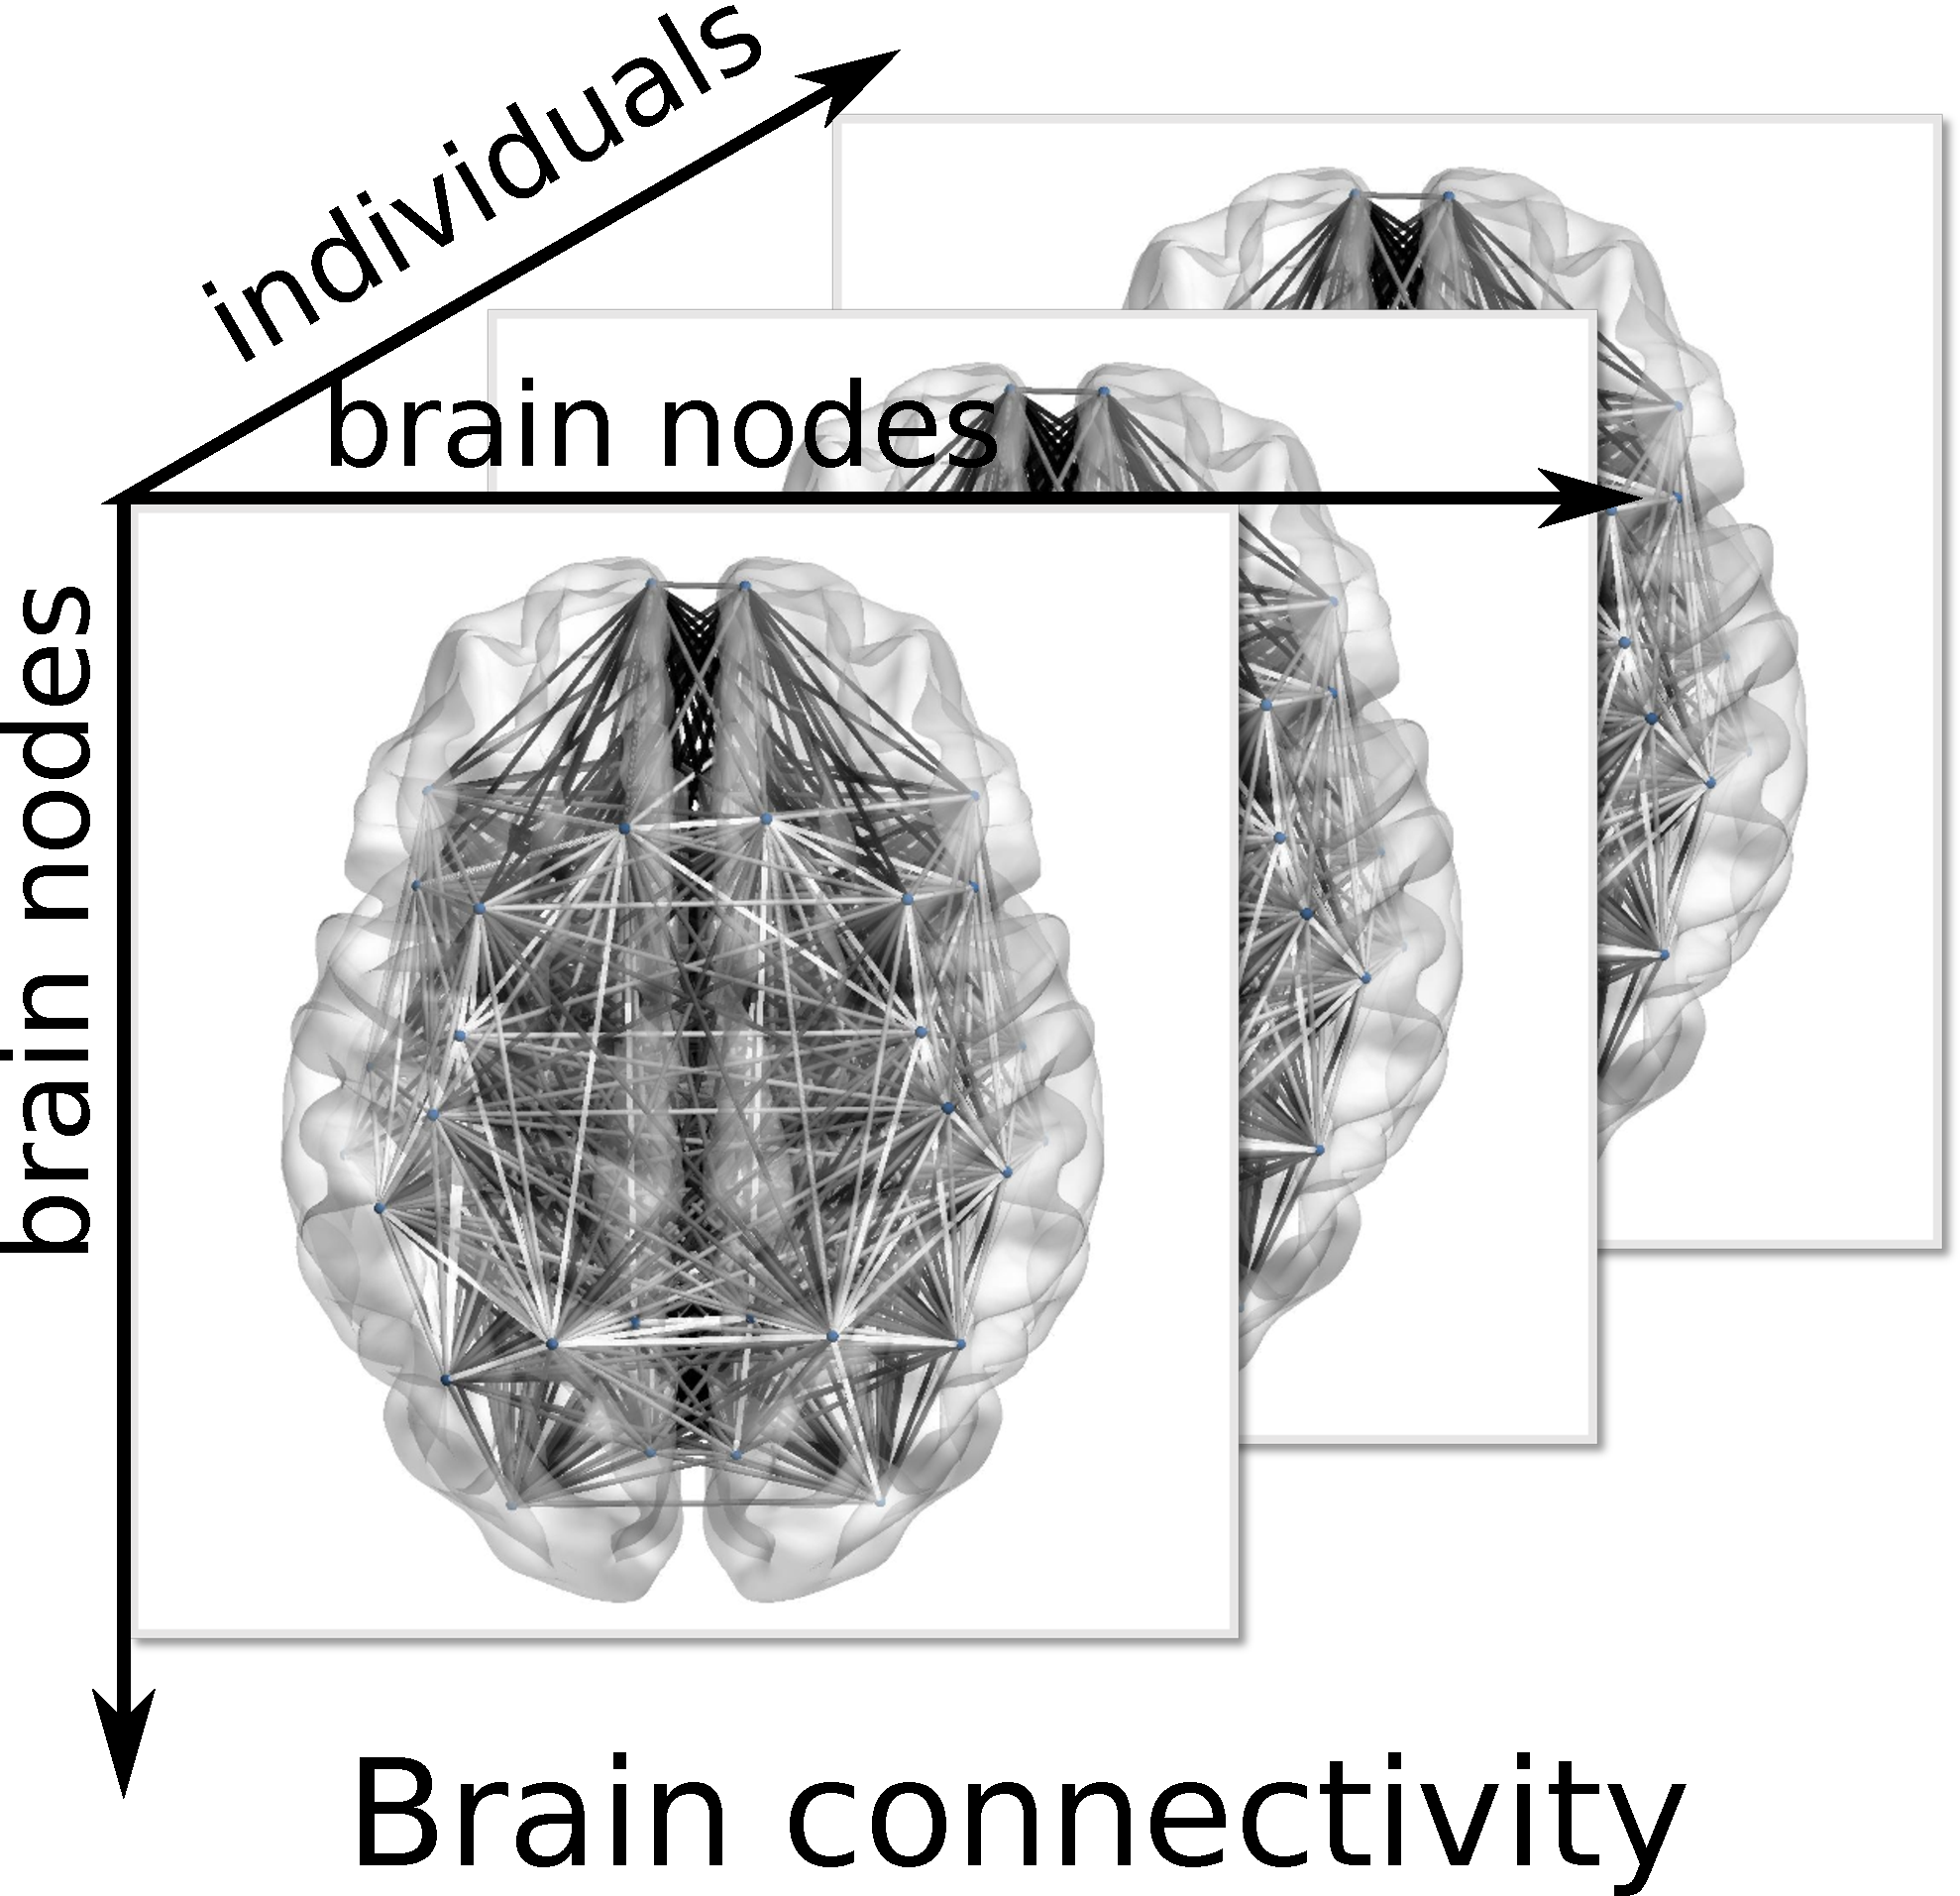
\includegraphics[width=\textwidth]{Figures/braindata.pdf}
     \end{center}
\end{column}
\begin{column}{0.7\textwidth} 
\begin{itemize}
    \item The human brain connectivity data consists of 68 brain regions for 114 individuals along with their IQ scores.
    \item  Data tensor $\tY\in\{0,1\}^{68\times68\times114}.$
\end{itemize}
\end{column}
\end{columns}

\begin{columns}
\begin{column}{0.6\textwidth}
 \begin{itemize}
     \item We examine the estimated signal tensor $\hat\Theta.$
     \item Top 10 brain edges based on regression analysis identifies inter-hemisphere connections.
 \end{itemize}
\end{column}
\begin{column}{0.4\textwidth} 
   \begin{center}
     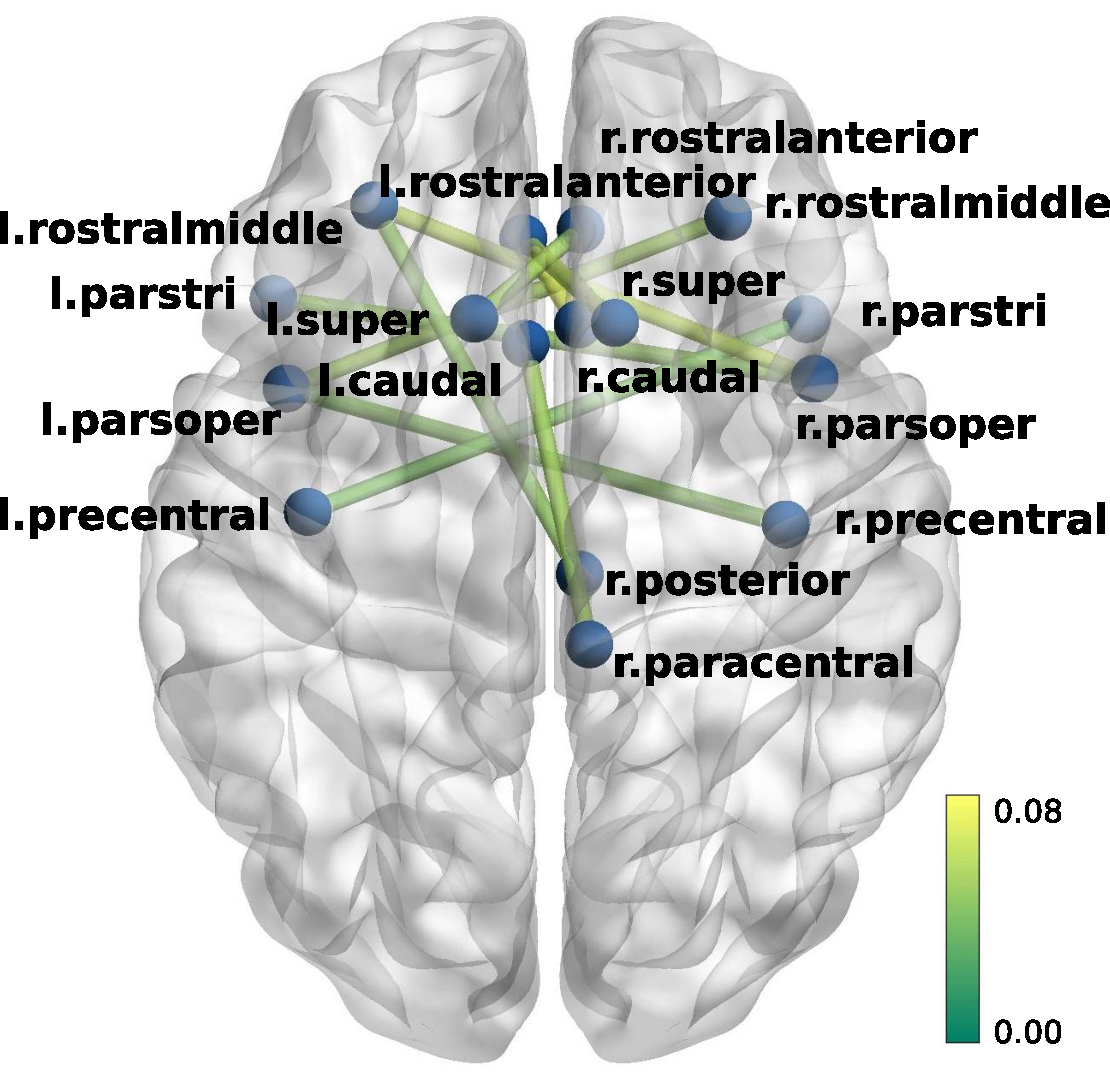
\includegraphics[width=\textwidth]{Figures/brainIQ.pdf}
     \end{center}
\end{column}
\end{columns}

\end{frame}



\begin{frame}{Data application: NIPS}
    \begin{columns}
\begin{column}{0.21\textwidth}
   \begin{center}
     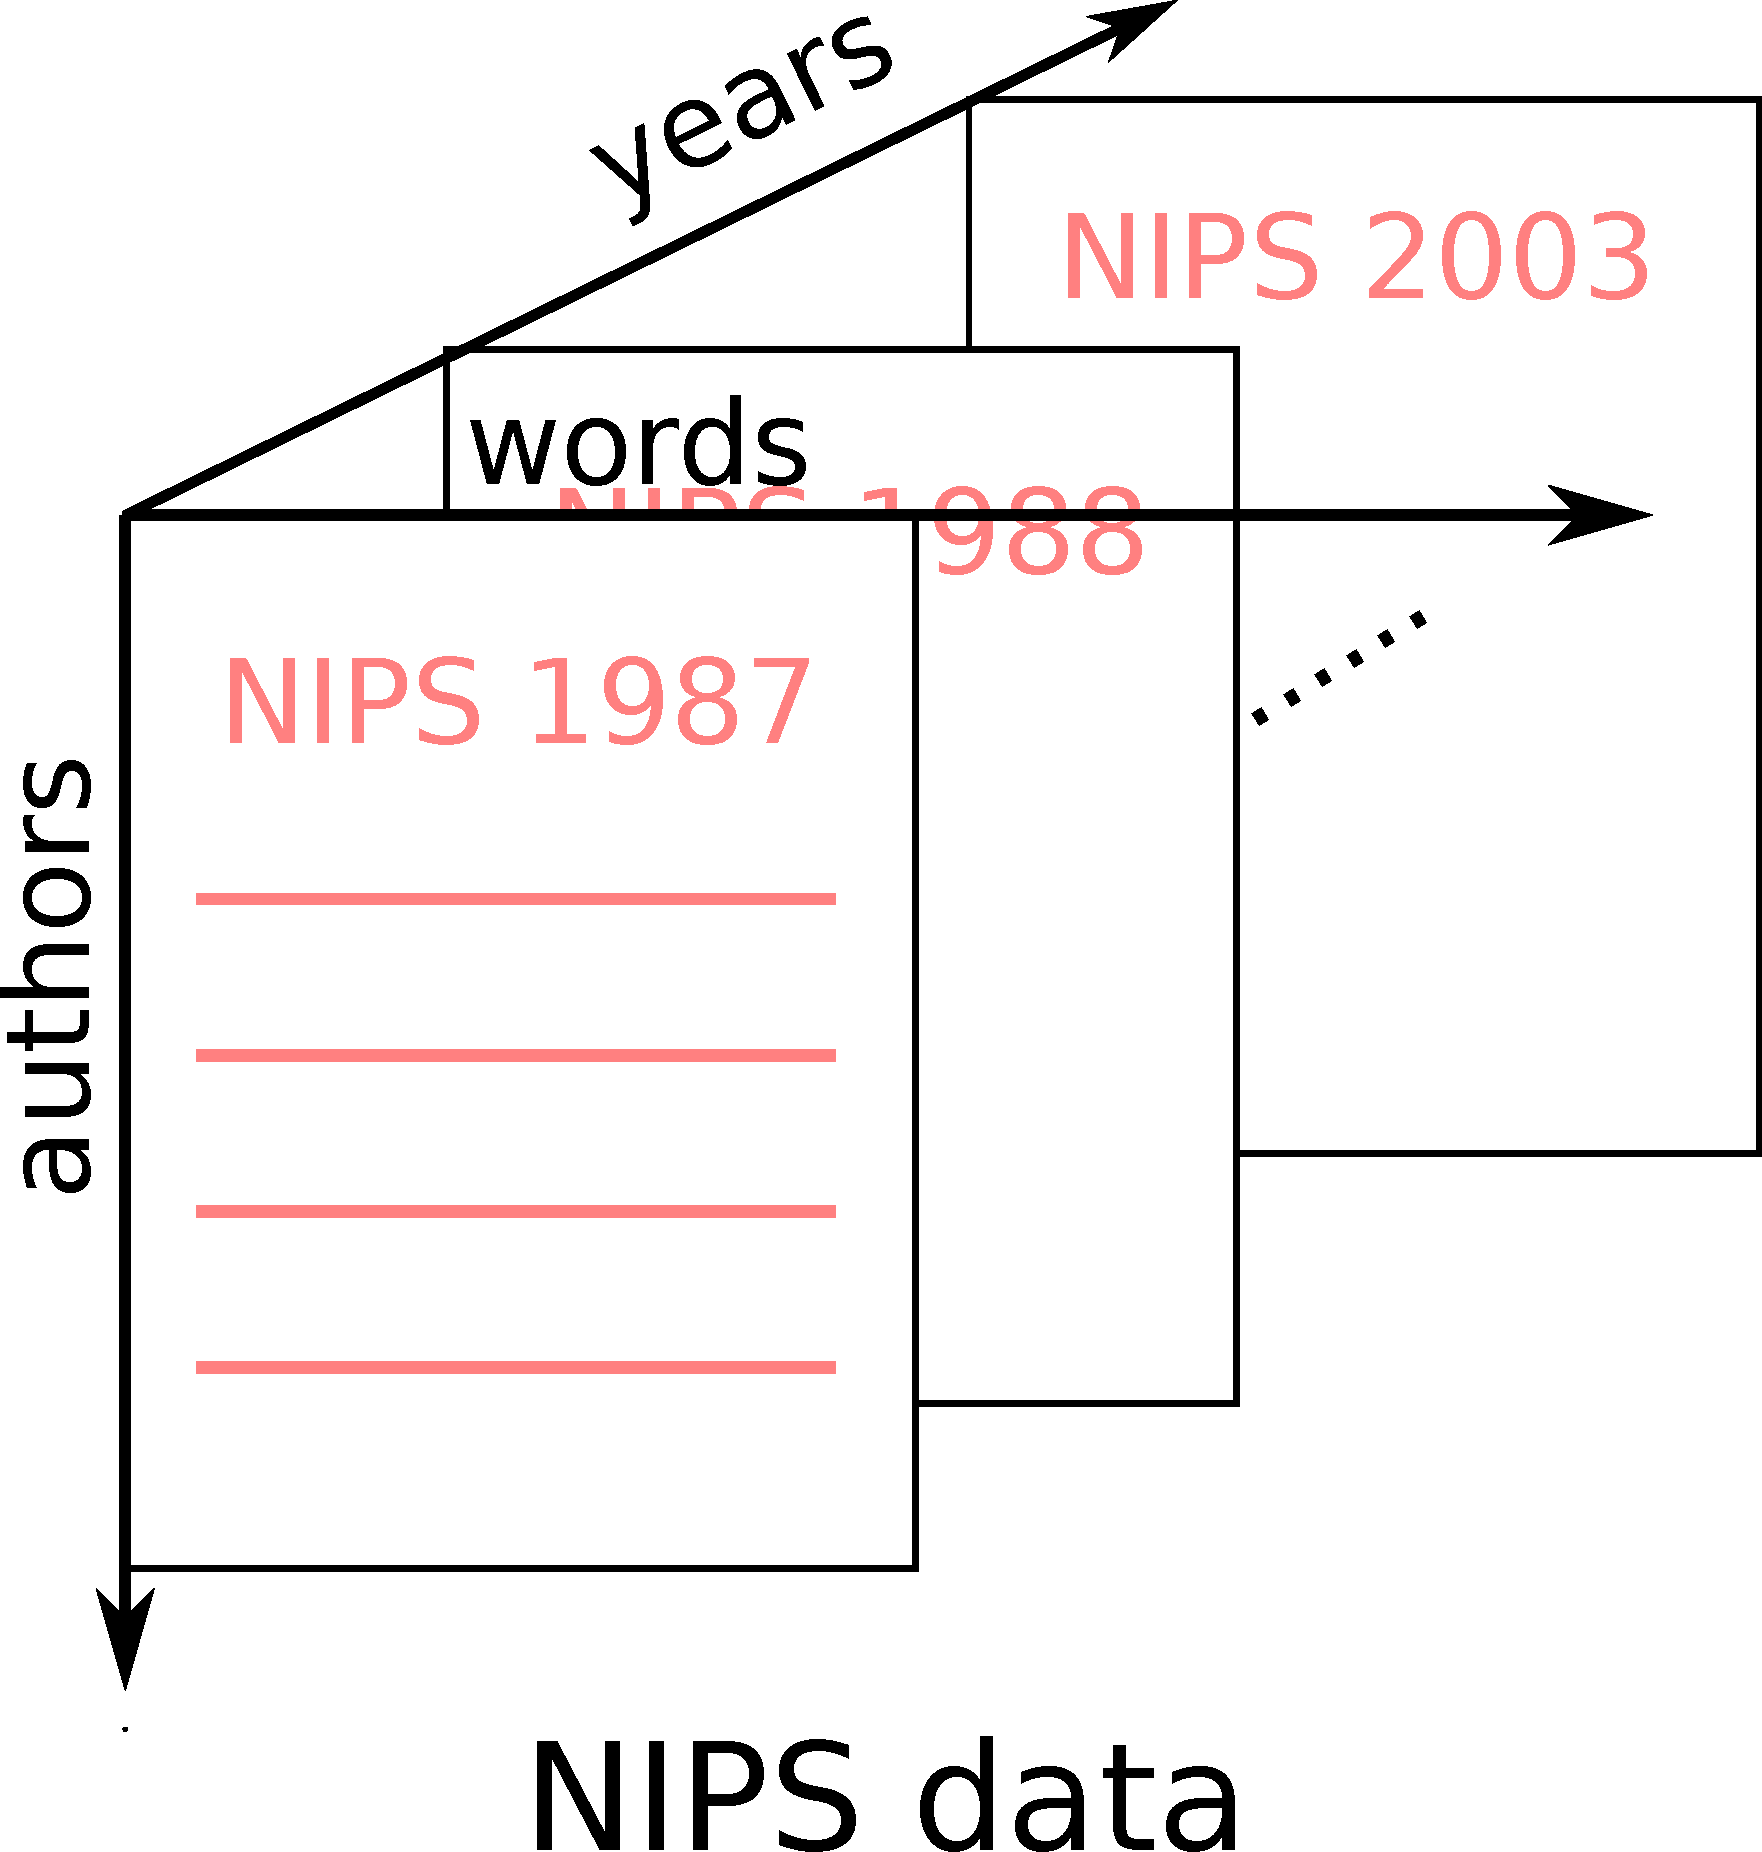
\includegraphics[width=\textwidth]{Figures/nipsdata.pdf}
     \end{center}
\end{column}
\begin{column}{0.7\textwidth} 
\begin{itemize}
    \item The NIPS dataset consists of word occurrence counts in papers published from 1987 to 2003.
    \item Data tensor $\tY\in\mathbb{R}^{100\times200\times17}.$ 
\end{itemize}
\end{column}
\end{columns}

\begin{columns}
\begin{column}{0.6\textwidth}
 \begin{itemize}
     \item We examine the estimated signal tensor $\hat\Theta.$
     \item Most frequent words are consistent with active topics in NIPS conference. 
     \item Strong heterogeneity among word occurrences across authors and years.
 \end{itemize}
\end{column}
\begin{column}{0.4\textwidth} 
   \begin{center}
     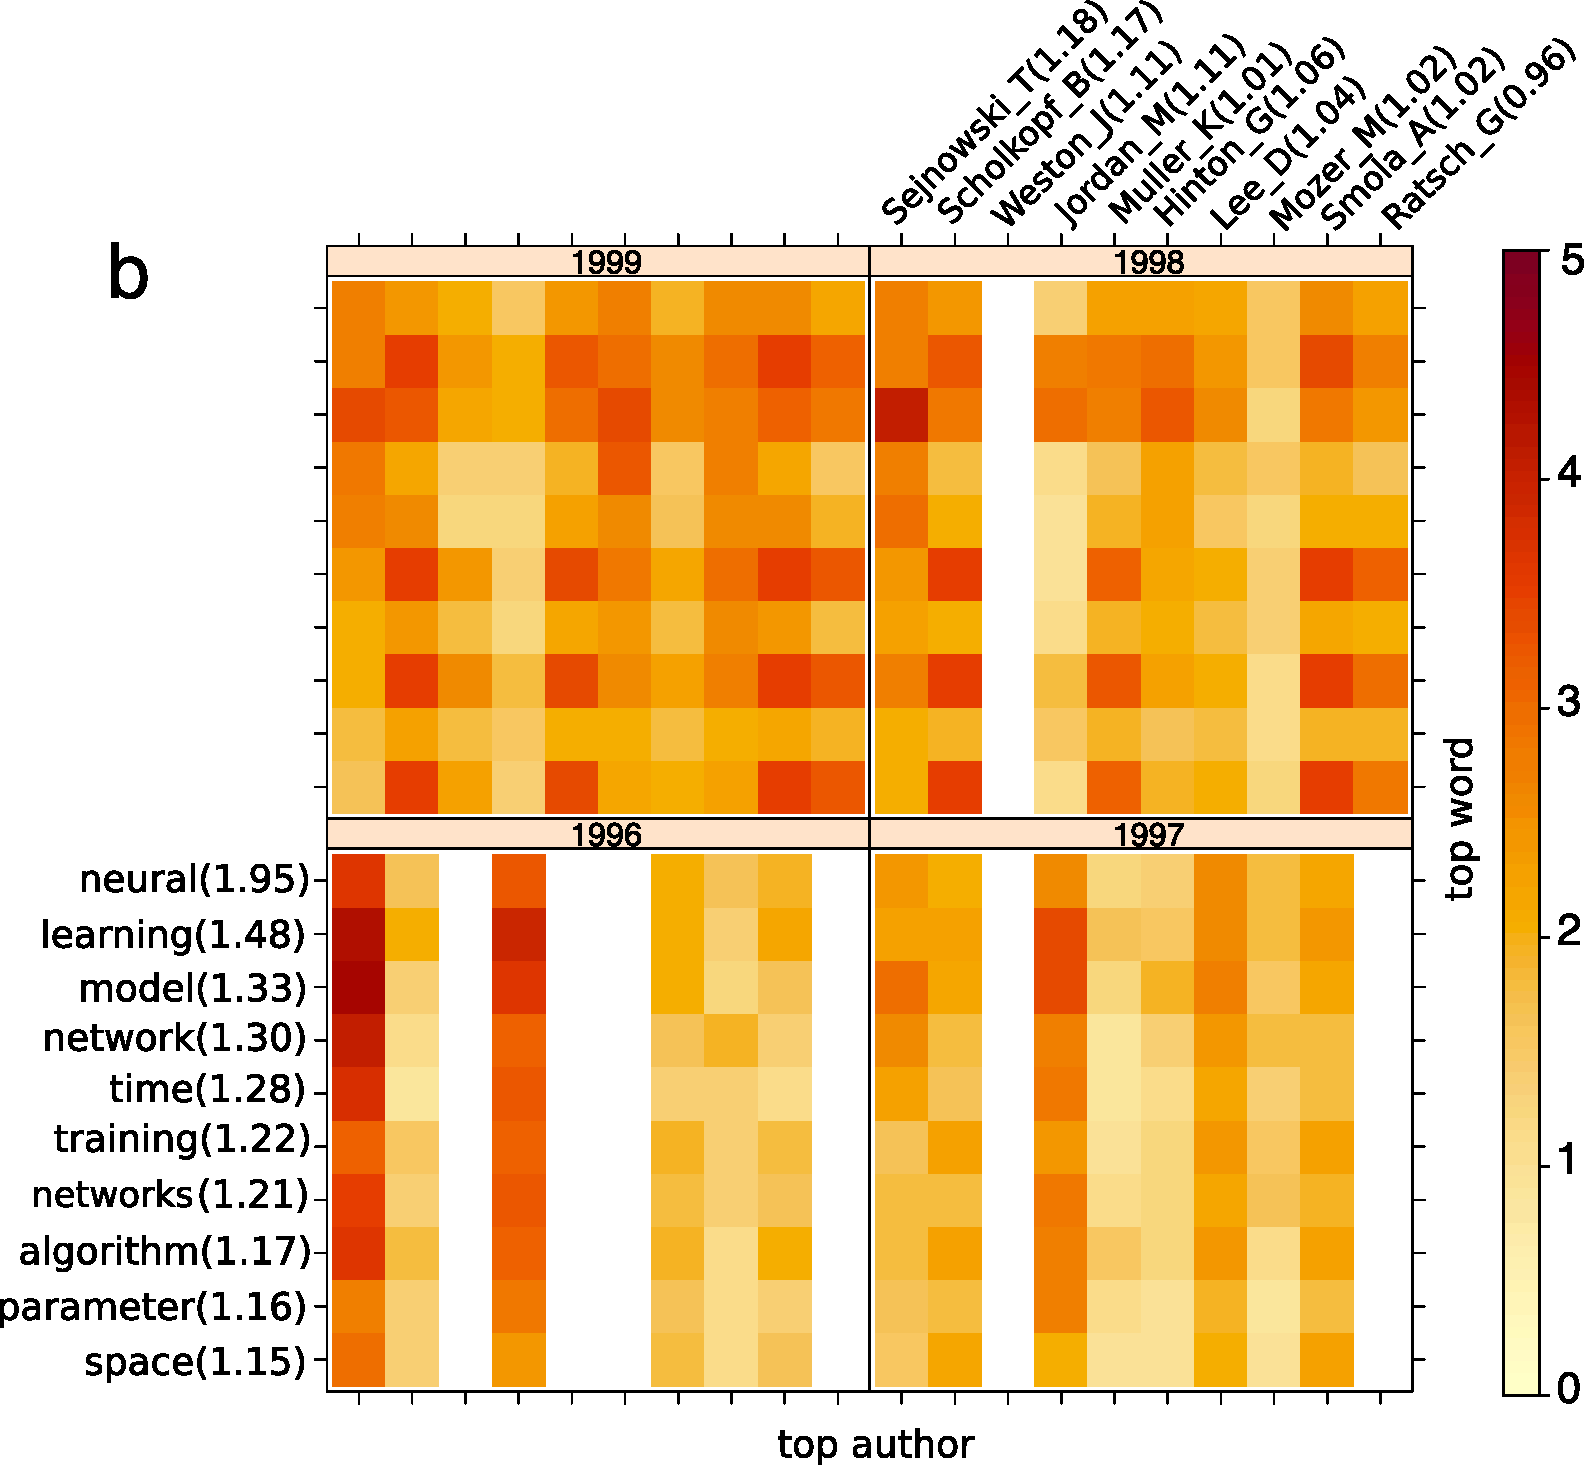
\includegraphics[width=\textwidth]{Figures/signal.pdf}
     \end{center}
\end{column}
\end{columns}
\end{frame}


\begin{frame}[label=result]{Data application: NIPS}
\begin{columns}
\begin{column}{0.5\textwidth} 
\scriptsize
\begin{itemize}
\item Top words: \emph{neural} (1.95), \emph{learning} (1.48), \emph{network} (1.21), \emph{training} (1.22), \emph{parameter (1.16)}.
\item Top authors: \emph{T. Sejnowski} (1.18), \emph{B. Sch\"{o}lkopf} (1.17), \emph{M. Jordan} (1.11), and \emph{G. Hinton} (1.06),
\item Top combinations: 
\\(\emph{\color{red}training}, \emph{\color{red}algorithm}) $\times$ (\emph{B. Sch\"{o}lkopf}, \emph{A. Smola}) $\times$ (1998, 1999), \\
(\emph{\color{blue}model}) $\times$ (\emph{M. Jordan}) $\times$ (1996).
\item Similar word patterns in 1998-1999:

(\emph{B. Sch\"{o}lkopf}, \emph{M\"{o}ller K}, \emph{A. Smola}, \emph{G. R\"{a}tsch}, \emph{J. Weston}) {\color{darkgreen}$\Rightarrow$ Co-authors}. 
\end{itemize}
\end{column}

\begin{column}{0.5\textwidth} 
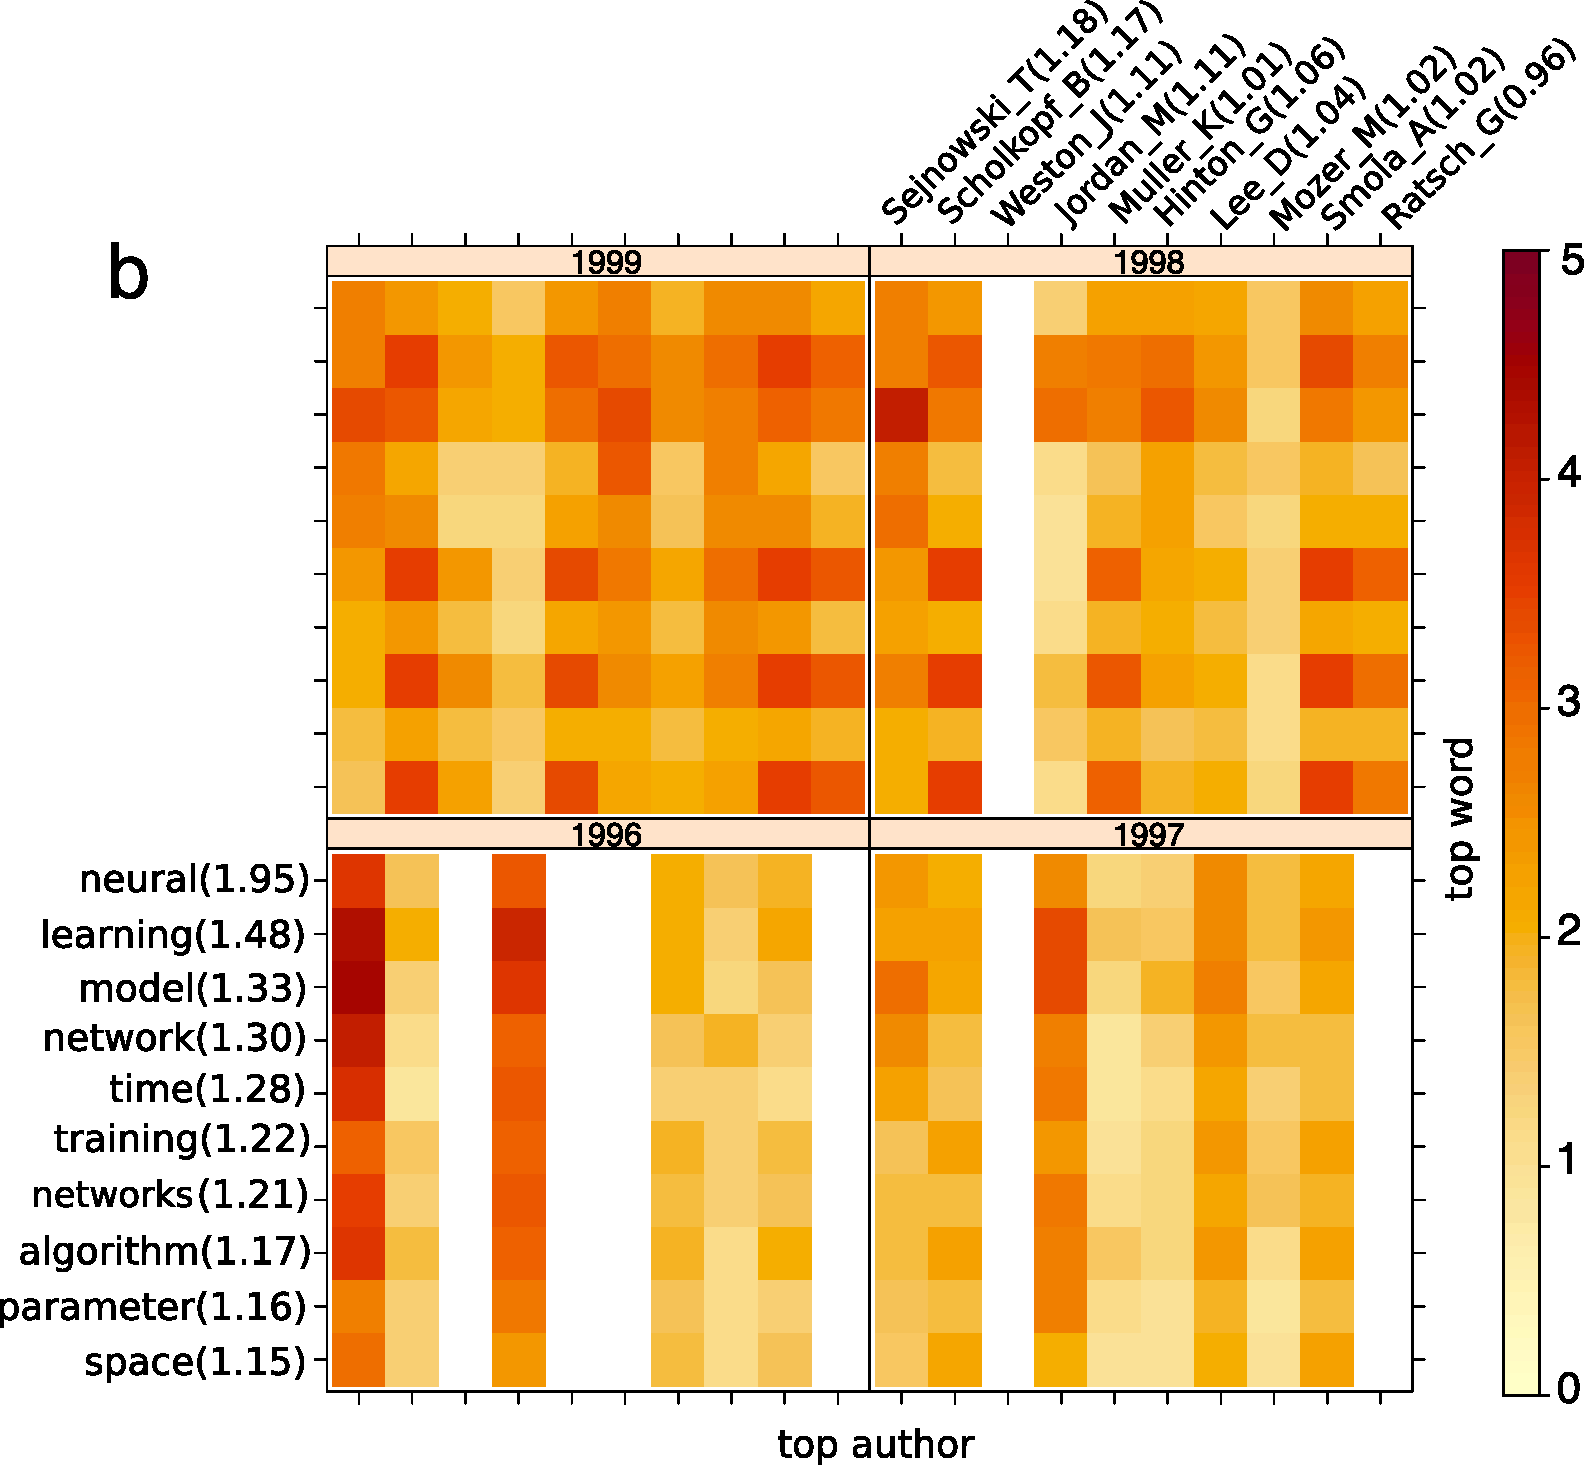
\includegraphics[width=1\textwidth]{Figures/signal.pdf}
\end{column}
\end{columns}

\vspace{1cm}
{\hfill \scriptsize Numbers in parentheses denote marginal averages based on $\hat \Theta$\\
\hfill \hyperlink{NIPS}{\beamerbutton{details}}
}
\end{frame}


\begin{frame}{Data application: Brain connectivity + NIPS}
\begin{itemize}
\item Our method achieves better test performance than low-rank methods. 
\end{itemize}
      \begin{center}
     \begin{table}
    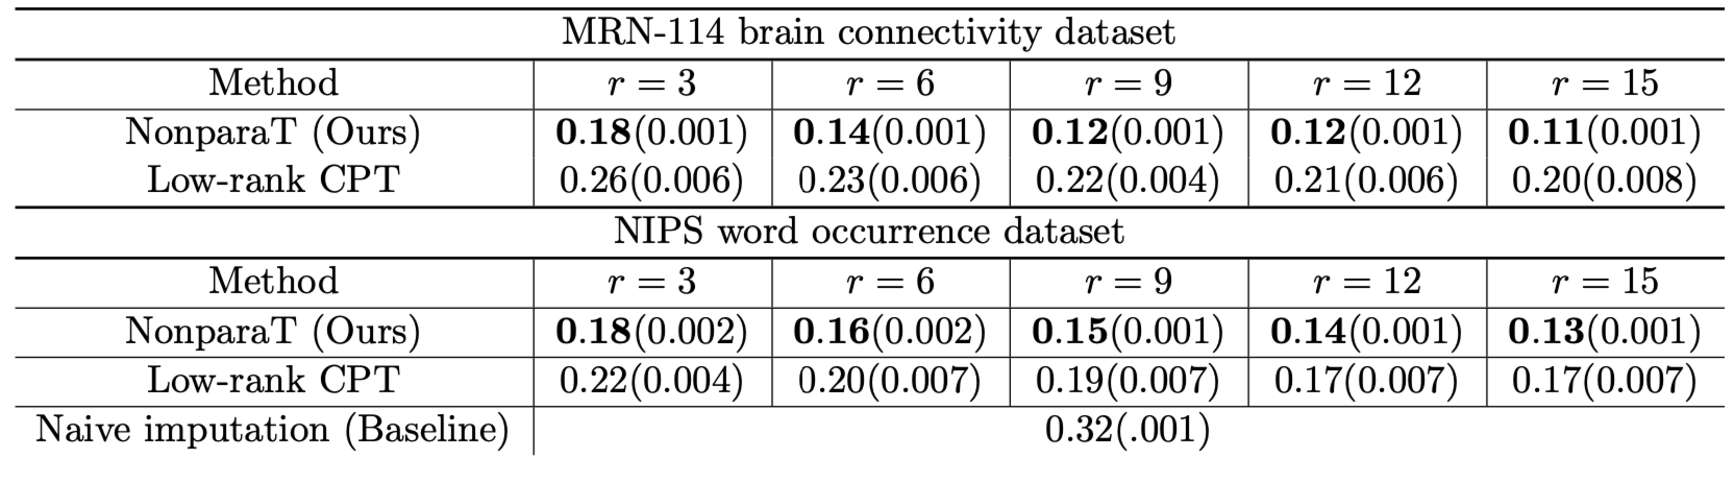
\includegraphics[width =\textwidth]{Figures/cvtable.pdf}
    \caption{\scriptsize MAE comparison in the brain data and NIPS data based on 5-folded cross-validations. Standard errors are reported in parenthesis.}
    \end{table}
    \end{center}
\end{frame}

\begin{frame}{Data application: Image}
 \begin{columns}
\begin{column}{0.20\textwidth}
   \begin{center}
     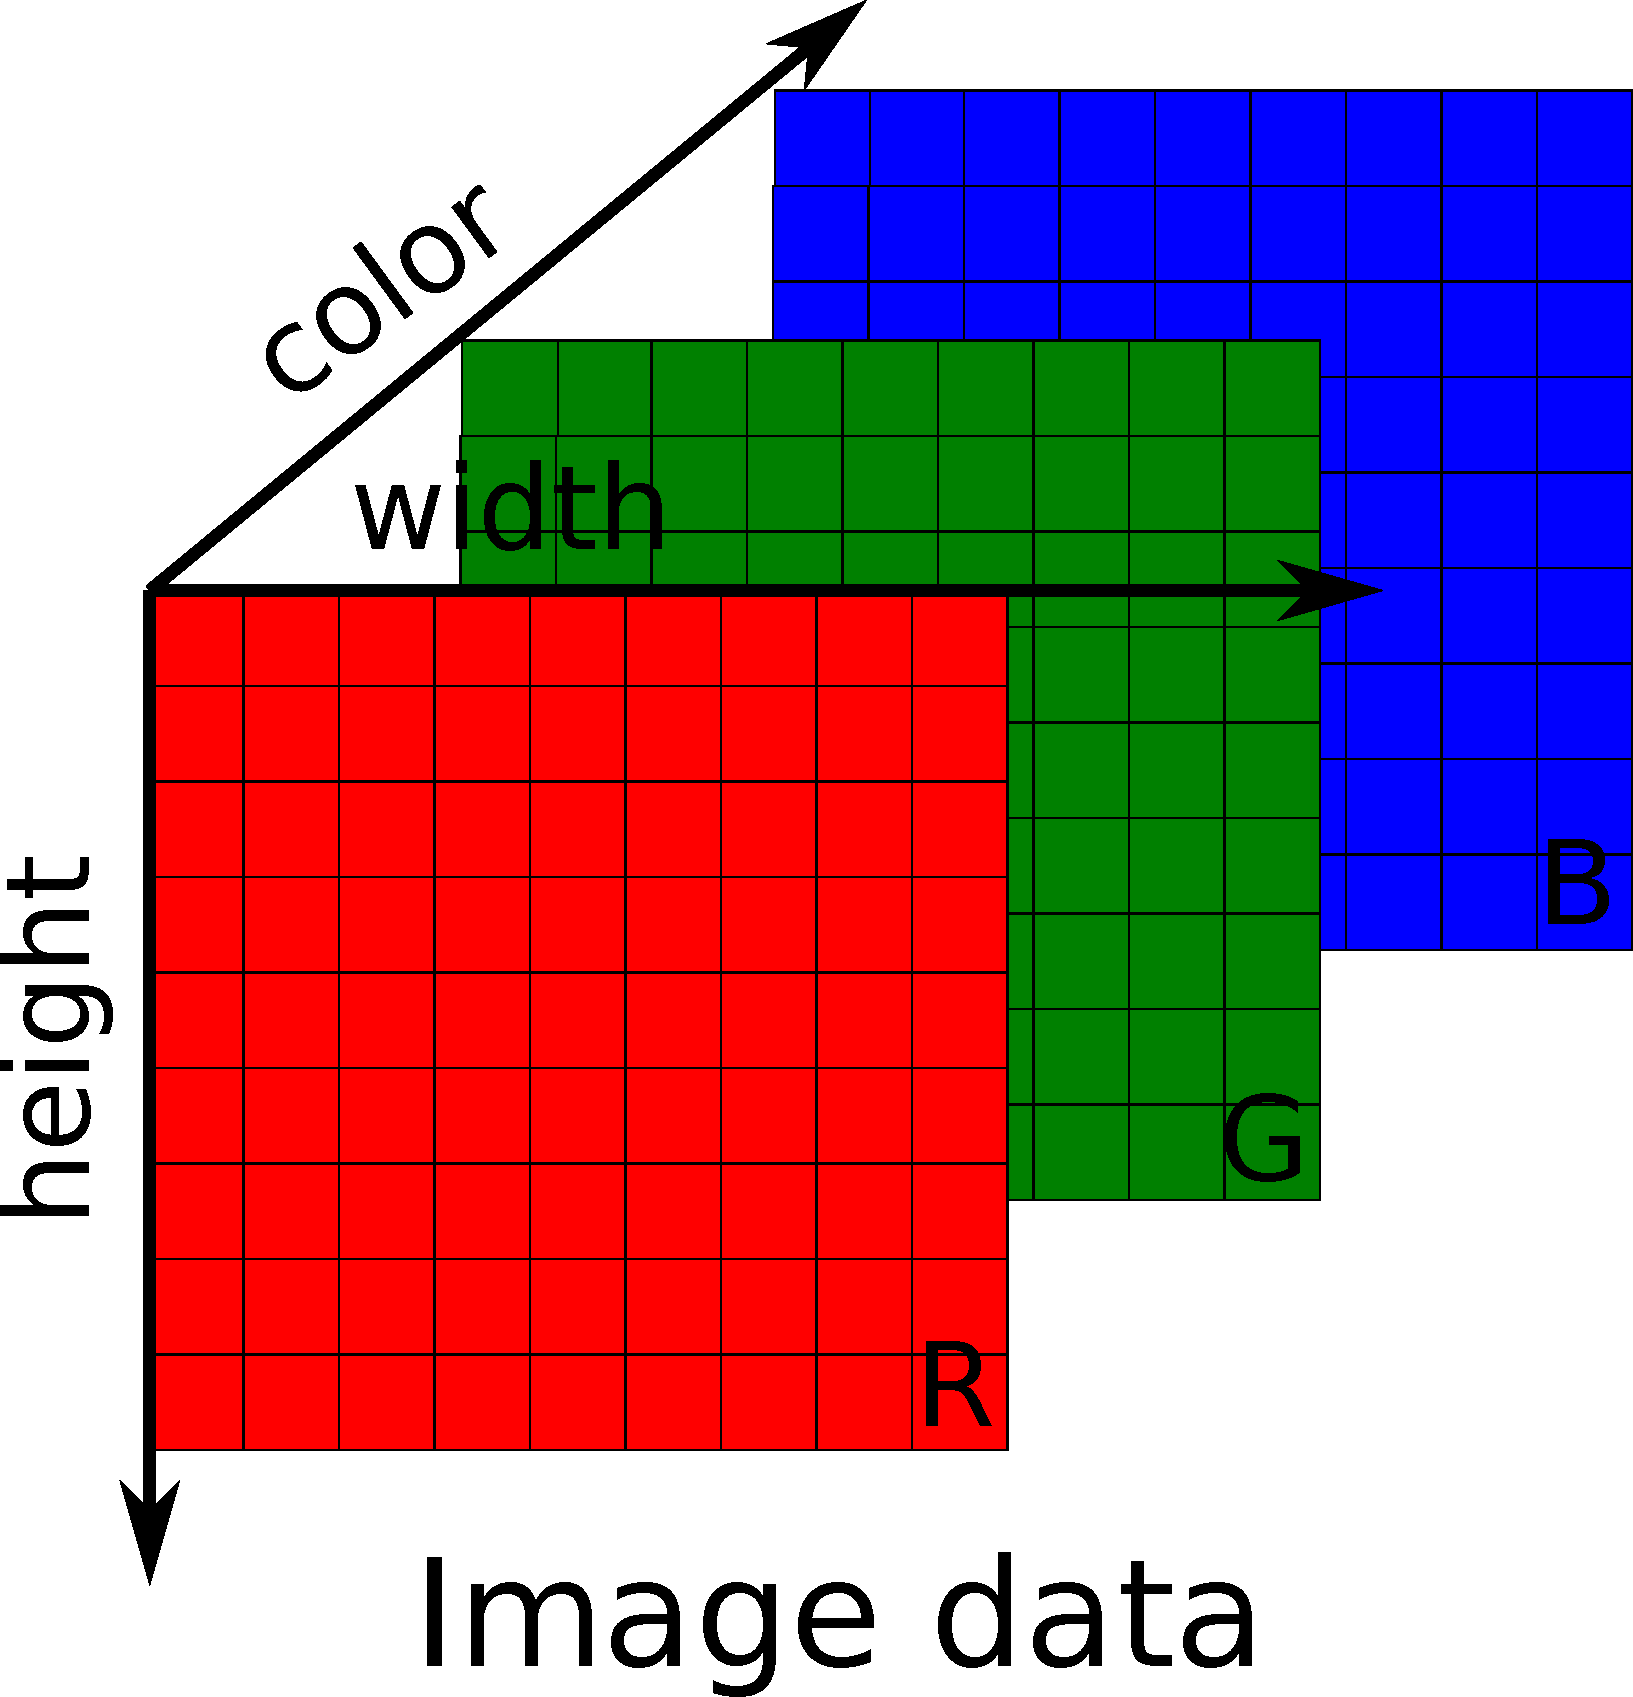
\includegraphics[width=\textwidth]{Figures/imgdata.pdf}
     \end{center}
\end{column}
\begin{column}{0.7\textwidth} 
\begin{itemize}
    \item The original data is from licensed google image file.
    \item Data tensor $\tY\in[0,1]^{217\times217\times3}.$ 
    \item We assess completion performance by sampling 50\% entries in the original image tensor.
\end{itemize}
\end{column}
\end{columns}


      \begin{center}
    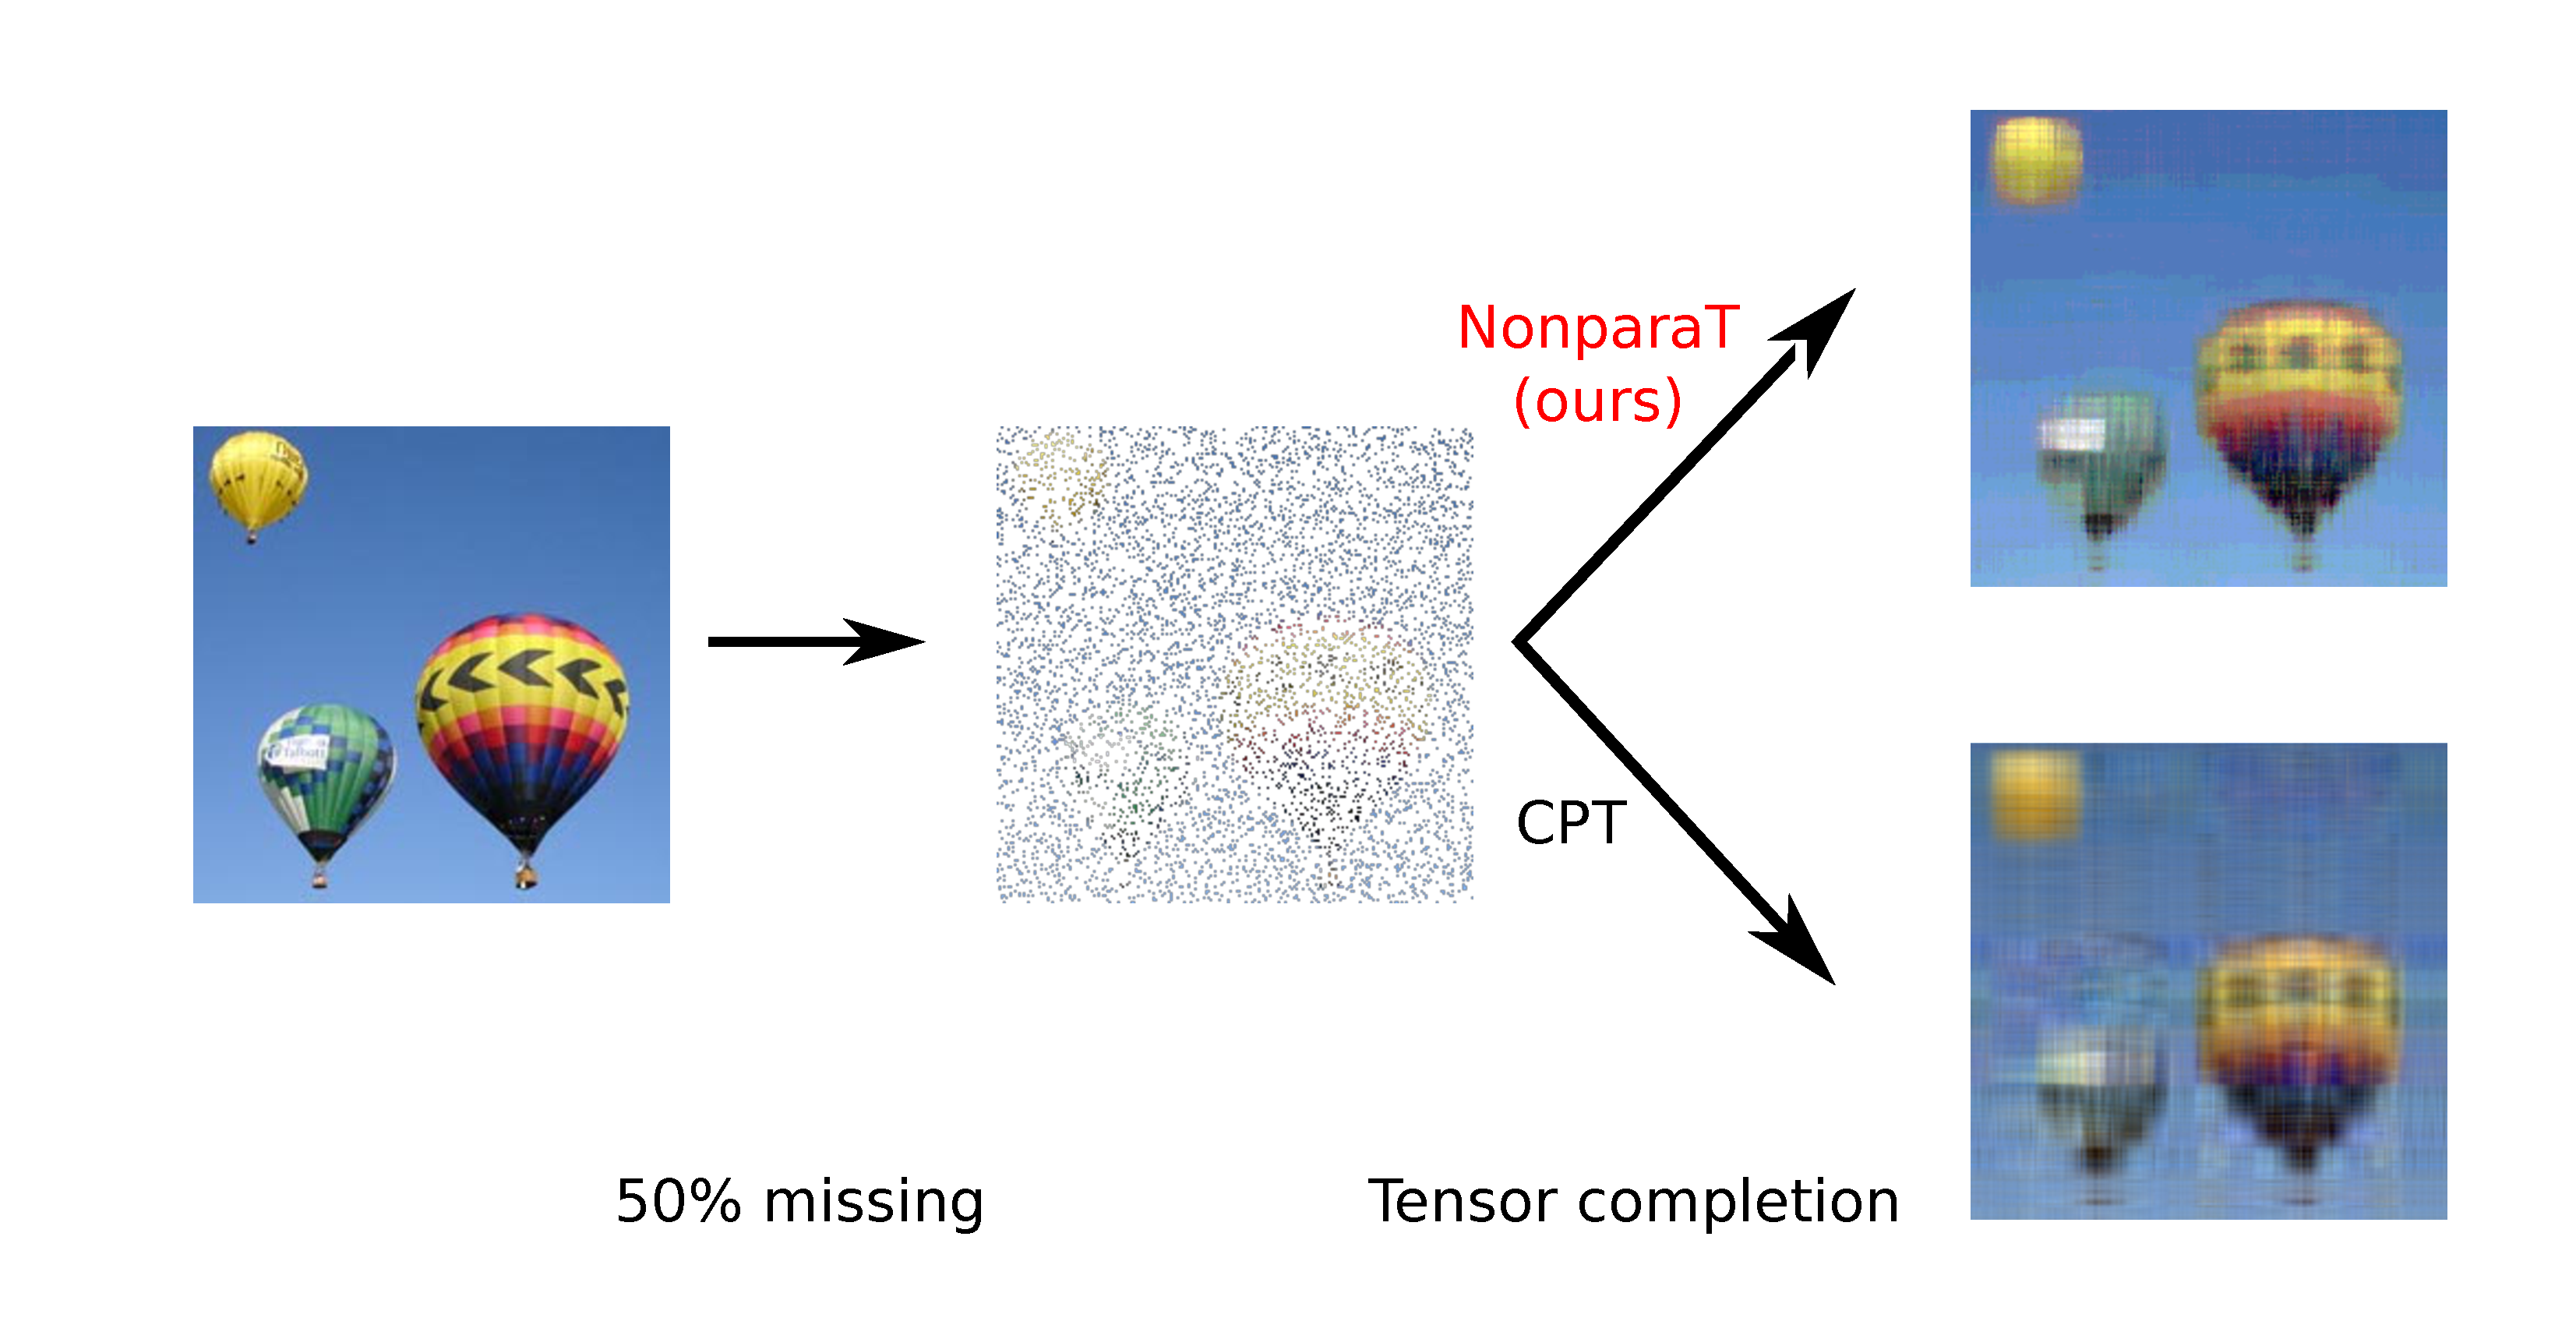
\includegraphics[width =\textwidth]{Figures/imageresult.pdf}
    \end{center}
\end{frame}


\begin{frame}{Summary}

Tensor analysis provides a rich source of
\begin{itemize}
\item fundamental problems in data science.
\item new tools for long-standing questions.
\item potentials for new applications.
\end{itemize}

\begin{block}{}
Our general strategy is to carve out a broad range of {\color{red}specially-structured tensors} that are useful in practice, and to develop efficient statistical methods for analyzing these high-dimensional tensor data.
\end{block}

References:
\begin{itemize}
\item {\color{blue}Beyond the signs: nonparametric tensor completion from sign series. \url{https://arxiv.org/pdf/2102.00384.pdf}}
\end{itemize}
\vspace{.2cm}
Acknowledgment: {\small NSF DMS 1915978 and Grant from Wisconsin Alumni Research Foundation.}
\end{frame}



\appendix
\begin{frame}{Appendix}
    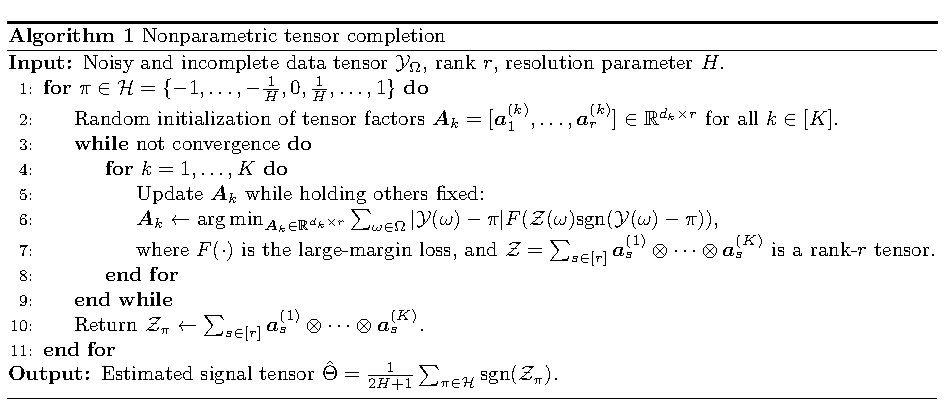
\includegraphics[width = \textwidth]{Figures/algorithm.pdf}
\end{frame}


\begin{frame}[label=NIPS]{Paper titles in NIPS dataset}
\tiny
1998:

\begin{itemize}
\item {\color{red} Kernel} PCA and De-Noising in Feature Spaces. Sebastian Mika, {\bf B. Sch\"{o}lkopf}, {\bf A. Smola}, {\bf K. M\"{u}ller}, M.\ Scholz, {\bf G.\ R\"{a}tsch}
\item  Shrinking the Tube: A New {\color{red} Support Vector Regression Algorithm}. {\bf B. Sch\"{o}lkopf}, P. Bartlett, {\bf A. Smola}, R. C. Williamson
\item Semiparametric {\color{red} Support Vector} and Linear Programming Machines. {\bf A. Smola}, T-T. Frieb, {\bf B. Sch\"{o}lkopf}
\item Regularizing AdaBoost. {\bf G. R\"{a}tsch}, T. Onoda, {\bf K. M\"{u}ller}
\end{itemize}

\bigskip

1999:
\begin{itemize}
\item v-Arc: Ensemble Learning in the Presence of Outliers. {\bf G. R\"{a}tsch}, {\bf B. Sch\"{o}lkopf}, {\bf A. Smola}, {\bf K. M\"{u}ller}, T. Onoda, S. Mika
\item Invariant Feature Extraction and Classification in Kernel Spaces. S. Mika, {\bf G. R\"{a}tsch}, {\bf J. Weston}, {\bf B. Sch\"{o}lkopf}, {\bf A. Smola}, {\bf K M\"{u}ller}
\item {\color{red} Support Vector Method} for Novelty Detection. {\bf B. Sch\"{o}lkopf}, R. C. Williamson, {\bf A. Smola}, J. S. Taylor, J. Platt.
\end{itemize}

\bigskip
1996:
\begin{itemize}
\item A Variational Principle for {\color{blue}Model}-based Morphing. L. Saul, {\bf M. Jordan}
\item Hidden Markov Decision Trees. {\bf M. Jordan}, Z. Ghahramani, L. Saul
\item Triangulation by Continuous Embedding. M. Meila, {\bf M. Jordan}
\item Recursive Algorithms for Approximating Probabilities in Graphical {\color{blue}Models}. T. Jaakkola, {\bf M. Jordan}
\end{itemize}


{\hfill \hyperlink{result}{\beamerbutton{Back to NIPS analysis}}}
\end{frame}

%\begin{frame}
%\frametitle{References}
%\tiny
%\begin{itemize}
%\item Oseledets, Ivan V. Tensor-train decomposition. SIAM Journal on Scientific Computing 33.5 (2011): 2295-2317.
%\item M. Wang and Y. Zeng. Multiway clustering via tensor block models. Advances in Neural Information Processing Systems 32 (NeurIPS), 715-725, 2019
%\item R. Han, Y. Luo, M. Wang, and A. R. Zhang. Exact clustering in tensor block model: Statistical optimality and computational limit. Under review, 2020.
%\end{itemize}



%\bibliography{tensor_wang}
%\end{frame}


\end{document}
